\documentclass[11pt]{article}

\usepackage[pdftex]{graphicx} % OU
% \usepackage[dvips]{graphicx}

% \usepackage[round]{natbib}
\usepackage{adjustbox,array,url,hyperref,multirow,makecell,tabularx,caption,subcaption}
% \usepackage{url,hyperref,multirow,makecell}
\usepackage[table]{xcolor}
\usepackage{lipsum}
\usepackage{cite}
\usepackage{amsfonts}
%\usepackage[latin1]{inputenc}
\usepackage[utf8]{inputenc}
%\usepackage[brazilian,brazil]{babel}
%\usepackage{apacite}
%\usepackage{float}
\usepackage{booktabs}
\usepackage{multirow}
\usepackage{multicol}
\usepackage{enumerate}
\usepackage[shortlabels]{enumitem}

\usepackage{todonotes}
\newcommand{\pmendes}[1]{\color{blue}\textbf{paulo says: }#1\color{black}}
\newcommand{\palan}[1]{\color{red}\textbf{alan says: }#1\color{black}}
\newcommand{\pdsm}[1]{\color{green}\textbf{daniel says: }#1\color{black}}

\usepackage{tikz}
\usetikzlibrary{
  angles,
  arrows,
  arrows.meta,
  calc,
  intersections,
  positioning,
  quotes,
  shapes.geometric,
  through,
}
\tikzset{
  x=0em,
  y=0em,
  node distance=1.2em,
  >=stealth',
}

\newcommand*\rot[1]{\rotatebox{90}{#1}}

\newtheorem{proposition}{Proposition}
\newtheorem{lemma}{Lemma}
\newtheorem{theorem}{Theorem}

\newcommand{\CQD}{\mbox{\rule[0pt]{1.5ex}{1.5ex}}\medskip}
\newcommand{\M}{\mathcal{M}}

\setlength{\oddsidemargin}{0.5cm} \setlength{\textwidth}{15cm}
\setlength{\topmargin}{-1.5cm} \setlength{\textheight}{22.3cm}%{24.7cm}

\usepackage{pdfpages}

\begin{document}

\LARGE

% \bigskip

%% TITLE
\begin{center}
{\bf Sensitive Content Detection in Video with Deep Learning
\Large
\\Dissertation}
\end{center}


\bigskip
\normalsize

\begin{flushright}

Pedro Vincius Almeida de Freitas\\
Pontifical Catholic University of Rio de Janeiro\\
\texttt{pedropva@telemidia.puc-rio.br}
\end{flushright}


\date{}

% $~$ \\

\thispagestyle{empty}

%
%
% Workaround for keywords. The keywords in the catalographic sheet must be separated by dots, while the ones shown in the abstract must be separated by semi-colons.
% Thats why we have two commands for each language: \keywords declares the keywords for the catalographic sheet, while \keywordsabstract declares the ones for the abstract.
\keywords
{
  \key{Conteúdo Sensível;}
  \key{Detecção de Conteúdo Sensível;}
  \key{Classificação Multimodal de Videos;}
  \key{Deep Learning.}
}

\keywordsabstract
{
  \key{Conteúdo Sensível;}
  \key{Detecção de Conteúdo Sensível;}
  \key{Classificação Multimodal de Videos;}
  \key{Deep Learning.}
}

\keywordsuk
{
  \key{Sensitive Content Detection;}
  \key{Sensitive Content Dataset;}
  \key{Multimodal Video Classification;}
  \key{Deep Learning.}
}

\keywordsabstractuk
{
  \key{Sensitive Content Detection;}
  \key{Sensitive Content Dataset;}
  \key{Multimodal Video Classification;}
  \key{Deep Learning.}
}

\abstract{
 \pva{RESUMO AQUI}
}

\abstractuk{
  \pva{ABSTRACT HERE}
}


% \newpage
\pagenumbering{roman} \setcounter{page}{-1}

% TABLE OF CONTENTS -  OPTIONAL
%\newpage
\tableofcontents

%% BEGIN DOCUMENT
\newpage
\pagenumbering{arabic} \setcounter{page}{1}


%%% Sections....

% Workaround for keywords. The keywords in the catalographic sheet must be separated by dots, while the ones shown in the abstract must be separated by semi-colons.
% Thats why we have two commands for each language: \keywords declares the keywords for the catalographic sheet, while \keywordsabstract declares the ones for the abstract.
\keywords
{
  \key{Conteúdo Sensível;}
  \key{Detecção de Conteúdo Sensível;}
  \key{Classificação Multimodal de Videos;}
  \key{Deep Learning.}
}

\keywordsabstract
{
  \key{Conteúdo Sensível;}
  \key{Detecção de Conteúdo Sensível;}
  \key{Classificação Multimodal de Videos;}
  \key{Deep Learning.}
}

\keywordsuk
{
  \key{Sensitive Content Detection;}
  \key{Sensitive Content Dataset;}
  \key{Multimodal Video Classification;}
  \key{Deep Learning.}
}

\keywordsabstractuk
{
  \key{Sensitive Content Detection;}
  \key{Sensitive Content Dataset;}
  \key{Multimodal Video Classification;}
  \key{Deep Learning.}
}

\abstract{
 \pva{RESUMO AQUI}
}

\abstractuk{
  \pva{ABSTRACT HERE}
}

%%% -*- coding: utf-8 -*-
\newpage

\chapter{Introduction}
\label{chap:introduction}

% INTRO SLR
The amount of multimedia content on the internet is increasing each year.
More than 300 hours of video are uploaded to YouTube every minute.\footnote{\url{https://biographon.com/youtube-stats}}
In this context, studies have shown that about 56\% of children between 10 and 13 years old have a smartphone \cite{remosoftware,chollet2017xception}, and 8 out of 10 teenagers have had a friend who shared some sensitive media through social networks such as Facebook, Twitter, and Whatsapp.\footnote{https://www.netnanny.com/the-importance-of-parental-control/}


% In Brazil, the ``Cicarely case'' was an example that forced youtube to be blocked.\footnote{\url{http://g1.globo.com/Noticias/Tecnologia/0,,AA1412609-6174-363,00.html}}
% In our research, we are interested in helping to avoid scenarios where pornography can be uploaded to education channels, which might expose students, sometimes underage, to this kind of content.\footnote{\url{https://g1.globo.com/sp/sao-paulo/noticia/2020/06/19/professor-de-etec-na-zona-norte-de-sp-e-afastado-apos-se-masturbar-durante-aula-virtual.ghtml}}. 
%This scenery presents challenges on controlling which kind of contents are uploaded to this storage and distribution services, while dealing with great amounts of videos.

This huge amount of data sharing pattern presents a challenge to the control of the type of content that is loaded to these video repositories. By allowing the upload of sensitive content from malicious users, content providers become exposed to legal issues. This is also a problem for users in those platforms, as they might get exposed to this content without a warning.

Methods based on \textit{Deep Learning} (DL) became the \textit{state-of-the-art} in various segments related to automatic video analysis. More specifically, 
Convolutional Neural Networks (CNN) architectures, or ConvNets, have become the primary method used for audio-visual pattern recognition.

The term \emph{Sensitive content} is often used as a reference to any media that contains content such as nudity, intense sexuality, violence, gore, and any other potentially disturbing or offensive subject.
On the other hand, a content is labeled as \emph{Safe} when that content is suitable for the general public.


% \begin{figure}[!ht]
%   \centering
%   \begin{subfigure}[b]{0.45\textwidth}
%     \centering
%     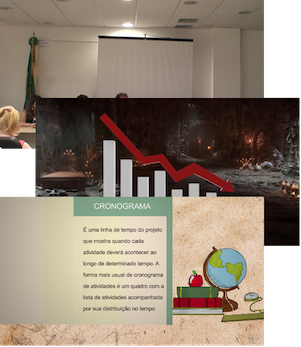
\includegraphics[width=0.8\textwidth]{img/safe.png}
%     \subcaption{Safe videos.}
%     \label{fig:samples_safe}
%   \end{subfigure}
%   \hspace{2em}
%   \begin{subfigure}[b]{0.45\textwidth}
%     \centering
%     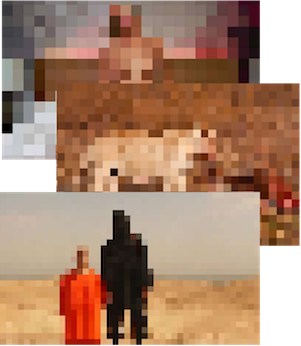
\includegraphics[width=0.8\textwidth]{img/sensitive.png}
%     \subcaption{Sensitive videos }
%     \label{fig:samples_not_save}
%   \end{subfigure}
%   \caption{Examples of Safe and Sensitive content.}
%   \label{fig:samples}
% \end{figure}
\begin{figure*}[!ht]
    \centering
    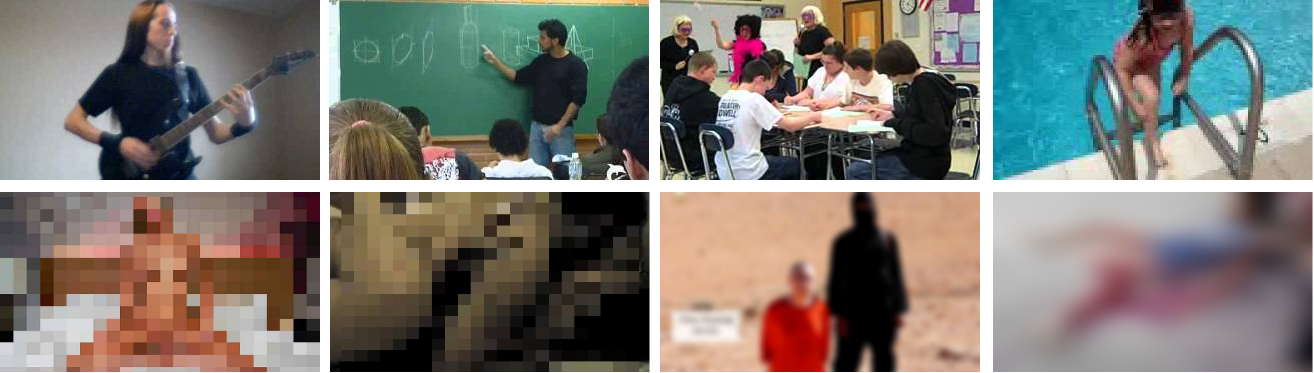
\includegraphics[width=0.95\textwidth]{img/safe-sensitive-horizontal.png}
    \caption{Examples of safe (top row) and sensitive videos (bottom row).}
    \label{fig:samples}
    \vspace{-1em}
\end{figure*}

Figure \ref{fig:samples} illustrates these two categories.
There are four scenes with safe content on the top row, and four scenes with sensitive content on the bottom row.

%As anyone can easily access any content on the Internet, whether exploring on search engines or through social networks, some groups of people (especially children) are very vulnerable to the exposure of content not suitable for their ages. 
%This situation calls for some media control strategy managed by parents or tutors, ensuring the least exposure to sensitive content.

%Controlling the type of content uploaded to video storage services requires an automatic analysis in an accurate and efficient way. 

%In this work, we created a CNN based model for video feature extraction and validate these video features experimenting with different baseline models to detect sensitive content.
%Then we evaluate the best model in a dataset created with videos sampled from the Brazilian RNP (National Research Network) repository video@RNP.\footnote{\url{https://www.video.rnp.br}}
%In our experimentation, the best model achieves a recall of 94.4\% and an F1-score of 95.6\% for pornography class.

Other works, such as \cite{moreira2019multimodal}, share our motivations and objectives, as described in Section \ref{chap:related}. However, most of them do not use both audio and image for classification. We use recent CNNs that have been showing great potential in video recognition and classification. Furthermore, none of them have the same definition of sensitive content as ours. For instance, the violence aspect of sensitive content in \cite{moreira2019multimodal} comprises any kind of physical violence, such as fights. In our definition, the violence aspect is defined by only extremely violent acts, such as torture, death, suicide, etc. %We also have created a large scale dataset that fits our definition of sensitive content.

Our work uses two CNNs: one to extract image sequence features and the other to extract audio features.
As we get one feature vector for each second of the video, we can approach the feature classification task as a time series classification, using a Recurrent Neural Network (RNN) as baseline. We also can combine those features to create a single feature vector for the entire video, which then is used as the input for other baseline classifiers.
%Our method uses a rather simpler approach for video classification and yet it still yields results significantly close to related works.


%\todo{Also talk about scene localization, scene detection}

%What is the difference between sensitive content detection and classification?

Although sometimes we may refer to the task we are addressing as sensitive content detection in video, our task is, specifically, binary classification of video: Finding out if sensitive content is or is not present in the video. 
Furthermore, since there is no frame-by-frame annotation, this dataset does not directly supports the task to find (either time-wise or space-wise) sensitive content in the video. 


%investigar a classifciacao e conteudo sensivel em video, principalmente em videos pornograficos e vi9lencia extrema

%objetivos espcificos
%cricao de dataset
%implemwentacao de baselines
%testar a eficiencia da extracao de features ja usada no yt8m
% testar a multimodalidade
% testar abordagem sequencial e não sequencial



%colocar exelpos do que é gore e oq n é 

%Obrigado pela recomendação professora! Foram excelentes leituras e tentarei trazer alguns desses conceitos para o meu trabalho.
% Infelizmente acho que nenhum dos datasets, apesar de numerosos e variados, é compativel com a nossa definição,

% O dataset que mais se aproximou com a nossa definição foi o MediaEval 2015, porém nosso dataset vem de principalmente de gravações amadoras ou CCTV, não de cenas cinematográficas.
% Seria interessante se testar se o treino em cenas amadoras se traduzem em bons resultados em cenas de estúdio, porém para fazer isso teriamos que filtrar alguns vídeos desse dataset que não entram em nossa definição.

% As nossas definições de violência são os vídeos de extremamente violentos (gore), que incluem pelo menos um desses: Sangue, Multilação e Morte.
% Não fazem parte da nossa definição: presença de armas, lutas, discussões, acidentes de carro (que não contenham nenhum dos topicos acima), violência emocional/mental e violência animada/cartunizada.

%In this work our goal is to create and validate a approach for sensitive content detection in video.

% Some of the questions we aim to answer with this work are:
% \begin{enumerate}
%     \item How does this approach compares with the related work?
%     \item What is the impact of also using audio in the model's performance?
%     \item Can the same model have a performance higher than 90\% on both pornography and violence detection tasks?
% \end{enumerate}

%To find the answers to these questions and fulfil our goal, 
The main contributions of this work are:
\begin{enumerate}
    % Criamos um dataset para a tarefa de classificacao de conteudo sensivel, o maior do mundo até onde sabemos
    \item To our knowledge, the largest sensitive content detection dataset.
    \item To our knowledge, we have obtained the best results in this task using only a generalistic feature extraction method and generic classifiers.
    % Testamos baselines nessa tarefa para validar o dataset e o funcionamento da extração de features
    \item We trained and tested baseline classifiers on the features extracted from our dataset in order to validate both the dataset and the efficiency nad operation of the genralistic feature extraction networks.  
    % Experimentamos com diferentes configurações de classificadores, inculsive sequenciais e naõ sequenciais
    \item We compared sequential and non sequential classifiers in this task.
    % Testamos a importancia dos features de imagem e de audio separadamente
    \item We tested the importance of image and audio features in this task.
    \item We also validate our approach by testing our best baseline in a well known pornography detection dataset, 2k-pornography. 
\end{enumerate}
Although the largest dataset for this task by our knowledge, our dataset is not manually labeled, which begs the question if it is noise-less enough for any training and evaluation in this task.  
Our intent is not to replace the 2k-pornography dataset, but to be a complement it, it still is the gold standard for pornography detection, in our dataset the videos were not manually labeled by a human, so we need to validate this dataset.

To perform this task, we created a large scale dataset, extracted features from this dataset using an generalist and well known feature extraction for video classification method, and performed experiments such as compare baseline classification models, compare which type of classification model (sequential or not) performs best, and compared the importance of audio and image features, further detailed in Chapter \ref{chap:method}.

This dissertation is organized as follows:
In Chapter \ref{chap:related} we discuss some of the related work.
In Chapter \ref{chap:theory} we present the theory behind some of the techniques behind the feature extraction method we used.
We present our dataset and metrics in Chapter \ref{chap:dataset}.
Then, in Chapter \ref{chap:method}, we present baseline models to detect sensitive content in videos.

Then, we evaluate and analyse our baseline models in Chapter \ref{chap:results}.
Finally, in Chapter \ref{chap:conclusions} we present, our conclusions, currently published papers, and future work.
Additionaly, in Appendix \ref{chap:appendix}, we show complementary data, such as tables, distributions and a dataset datasheet.
\section{Related Work}
\label{sec:related}
% VARIFICAR: https://www.sciencedirect.com/science/article/pii/S0925231217312493

% commented out because wqe have a more recent paper from theese same authors
%Song and Kin~\cite{song2018pornographic} create a scheme for detecting pornography videos using multimodal features: Image descriptor features of the frame sequence, extracted using the VGG-16 CNN\cite{vgg}, motion features extracted using optical flow\cite{opticalflow}, and audio features extracted using a Mel-scaled spectrogram.
%The final features for each model are obtained by an average pooling of each of the features by a sample in the video.
%Each of those kinds of features is used in a single SVM classifier per type of feature, resulting in an image sequence-based detector, a motion-based detector, and an audio-based detector.
%The final decision-making is done by model stacking all detectors.
%The authors used a modified dataset based on the 2k-pornography dataset\cite{2kdataset} for training and testing.
%The results of their method are an average of 63.4\% with a 100\% true positive rate for porn, and an average of 23.5\% of the false-positive rate. 
%Our work also uses multimodal features, but we only use image sequence features and audio features, furthermore, we use an Inception-V3 CNN instead of the VGG-16 CNN for extracting image sequence features and use an Audio VGG CNN for extracting audio features.
%Although the authors achieve 100\% recall rate for pornography, which is the main goal of their task, their model also has a 23.5\% false-positive rate, which means that normal videos would be occasionally classified as pornography.
%Our aim is to also have a true positive rate as high as theirs, while still further reducing the false positive rate.

Castro~\cite{torres2018automatic} shows an implementation of a pornography video classifier using a convolutional neural network from Open pornography\cite{mahadeokar2016open}.
The CNN does a logistic regression on each frame, resulting in a value from 0 to 1 at each frame.
The higher the value is, the higher is the likelihood of the frame being pornography.
The dataset used contained 90 non-pornography video segments and 89 pornography video segments extracted from 11 movies.
The final score for the video the max value from all frames of the video.
The experiment showed an accuracy of 81\%, F1-score, and Matthew’s correlation coefficient(MCC) for the pornography class of 0.8047 and 0.6343, respectively.
%Although the work also approaches pornography content detection in videos problem with CNN like ours, it does not make use of audio features.
%The method is also different, it performs the regression first, then it takes the max value from all frames of the video, while ours combines features from all frames of the video into a single vector of features(by averaging) and then performs classification on the resulting features.

Wehrmann \textit{et al.}~\cite{wehrmann2018adult} classify adult content trained on the NPDI video dataset, which consists of 802 videos, totaling 80 hours of videos, half of them with adult content.
Those videos were processed by keyframes, varying between 1 and 320 frames per video.
The selected keyframes of each video were chosen by a scene segmentation algorithm, resulting in 16727 images.
Their architecture consists of a Convolutional Network and an LSTM~\cite{hochreiter1997long} (Long-Short Term Memory).
Those models were chosen for feature extraction with CNN and sequence learning with LSTM, taking into consideration modifications on the images such as scaling and distorting.
Using this approach the authors achieved a score of 95.3\% accuracy using a ROC curve as an evaluation criterion.
%In our model, we also approached the video analysis using frame by frame processing, but we chose evenly spaced frames by their timestamps, not a segmentation algorithm.
%We also processed the extracted sound and image embeddings from each frame using a pre-trained Convolutional Neural Network, instead of an untrained one.
%\hl{Resulting in an accuracy of 98\% and 97.97\% F1-score for pornography class.}

Sing \textit{at. al.}\cite{singh2019kidsguard} proposes a fine-grained approach for child unsafe video representation and detection. One of its main objectives is to optimize detection on sparsely present child unsafe content and it does so by using a VGG16\cite{vgg} Convolutional Neural Network (CNN) to encode each frame, at 1-second granularity, in 512 real values. 
Then an LSTM autoencoder is trained to output the sequence backward on those encoded frames. 
Once the LSTM autoencoder is trained, then a fully connected layer of neurons is used to fine-tune and classify each frame. 
The dataset used comprises 109,835 short-duration video clips extracted from four animes. 
The results for binary classification using safe and unsafe classes were 81\% recall for unsafe and 80\% recall for safe class.
%Although this work also has similar objectives as ours and also uses a CNN-based encoding method, ours uses both visual and auditive features to encode a video. 
%Their work uses 1 frame per second granularity and ours has the same encoding rate. The main differences between both works are on the dataset: Theirs consists of small clips of only anime videos. Ours also uses other types of videos such as live-action and other animations. 
%In our dataset, the length of videos range from 6 seconds to 30 minutes.

Song \textit{at. al.}~\cite{song2020enhanced} proposed a multimodal stacking scheme for quick and accurate online detection of pornographic content.
Their work uses both visual and auditory features as input for their detection method. 
They use a VGG16 model and a bi-directional Recurrent Neural Network (RNN) to extract visual features and a combination of a Mel-scaled spectrogram followed by multilayered dilated convolutions to extract audio features. 
Using only the visual and auditory features, a video classifier and an audio classifier are trained, respectively. 
By using both features together, one fusion classifier is also trained.
Then, these three component classifiers are combined in an ensemble scheme to reduce the false-negative errors and for faster detection. 
The proposed detection method yields a true positive rate of 95.40\% and a false negative rate of 4.60\% on the pornography class, totaling a recall for the pornography class of 95.40\%. 
The dataset used was the pornography-2k\cite{2kdataset} dataset plus examples of videos with only pornographic or non-pornographic audio collected by the authors. 
% This work is similar to ours because it also uses a multimodal approach to detection, albeit ours is not for pornography detection only.
% It also uses the same sampling rate of a frame for each second and uses a deep learning method for extracting high-level features, which are then classified by one or more machine learning models. 
% Our work has a different dataset, comprised of pornography, gore, and violent videos for the inappropriate class and miscellaneous and educational YouTube videos as an appropriate class. 
% We also use different feature extraction methods for image and audio features. 
% Finally, in contrast with their ensemble approach, we use a single SVM model to classify the extracted features from our dataset.

Moreira \textit{et.al.}~\cite{moreira2019multimodal} has similar detection focuses as ours: Pornography and violence. 
Their method uses four multi-modal classifiers, two for audio and two for image, those classifiers were fed features from multiple handcrafted feature extraction methods. Their work also allows for sensitive scene localization and is geared towards mobile device applications.
%Our uses Deep Learning to extract high-level features and uses one classifier for both aggregation and classification of the features. 
The authors propose a method for sensitive scene localization which uses the output of four multi-modal classifiers on snippets of the video, then creates a fusion vector at each second of the video. 
Finally, they test different classifiers on the fusion vector for each task: detecting pornography and detecting violence. Their best result on the pornography task was 90.75\% accuracy and 93.53\% on the F2 metric. For the violent videos, they achieved 0.502 on the MAP2014 evaluation metric.
%Some differences between this work and our are mainly its objectives: To detect if and at what time the sensitive video occurs. 
%While our only objective is to detect if there is or not sensitive content in a video. Our definition of violent videos consists of extremely violent videos, while theirs also considers fights and hat-speech. Other differences stand out as the dataset and the methods used for feature extraction and classification. 
%We use an author-made dataset and investigate what result of a deep learning-based approach to this problem can yield.

%THEIR METHOD'S FINAL USER IS A PERSON USING A MOBILE DEVICE, OUR METHOD IS AIMED TO VIDEO HOSTING PLATFORMS, NOT USERS}

%THEIR METHOD EVALUATES ON EACH FRAME, OUR ON THE ENTIRE VIDEO}

The paper "Porn Streamer Recognition in Live Video Streaming via Attention-Gated Multimodal Deep Features"~\cite{wang2019porn} proposes a pornography method for use in live streams, focusing on real-time processing, their work uses multimodal features, namely, image, audio, and optical flow~\cite{horn1981opticalflow}. 
An Xception~\cite{chollet2017xception} model is used to extract spatial features from keyframes. 
To get the optical flow frames, they also use a CNN to extract the optical flow from the video, then, use another Xception model to extract the high-level optical flow features. 
Finally, they use a short-time Fourier transformation to create spectrograms and feed those spectrograms to a third Xception model and thus acquiring the extracted audio features.  
Each of the multimodal features extracted then is passed onto bidirectional GRUs\cite{dey2017GRU}, to obtain temporal context, then, to create a better-unified representation, all the features go through three interconnected Attention-gated layers, each with three Attention-gated units proposed in the paper. After obtaining the dense representation of the input types, it is applied a fully connected layer of neurons with \textit{softmax} function. Their work archives 76.33\% accuracy and runs at 66.1 fps.
%In our work, we strive for detecting both violence and pornography, we use only two types of input data, image, and audio, and we use a specific CNN for each type of data, while their work focused only on detecting pornography and used the same CNN model for all three types of input. 
%We investigate whether bigger and more specialized models can create better high-level features and further increase the quality of classification.

Liu \textit{et. al.} ~\cite{liu2020analyzing} proposes a multi-modal approach to pornography detection, it uses audio-frames and visual-frames to create handcrafted low-level features based on, respectively, periodic patterns and salient regions. Once those features are extracted, they use k-means clustering to create audio and visual codebooks. 
Then, low-level audio and visual features of test videos are converted into mid-level semantic histograms via de audio or visual codebook. 
Finally, the histograms are concatenated to represent the video and a periodicity-based video decision algorithm is used to fuse the classification results of multi-modal codebooks and the results of an SVM trained on the concatenated mid-level semantic features train set.
The true positive rate of their approach achieves 96.7\% while the false positive rate is about 10\%.
%Liu \textit{et. al.} detects pornography, they do not detect violence, and also use handcrafted features such as Region Of Interest (ROI) extraction and skin-color segmentation.
%Whereas our approach uses a fully automatic feature extraction method based on CNNs and our feature fusion method consists of just a concatenation followed by a classifier.

%Although most of the aforementioned works also approach pornography detection in videos but do not consider violent videos like ours.
Most related works focus on pornography detection alone, while ours aims at detecting either pornographic or violent content. Moreover, some of them only use image-frame features, whereas we use both audio and image-frame features. We also use deep learning feature extraction methods instead of hand-crafted ones.
Finally, a central difference is our dataset: Ours contains violent scenes and is significantly larger than most datasets used on other related works.
%%% -*- coding: utf-8 -*-
\newpage

\chapter{Theory and technical background}
\label{chap:theory}

This Chapter aims to set a basic understanding the concepts underlying the techniques used in this Dissertation.

\section{Artificial Neural Networks}\label{sec:NNs}

Artificial Neural Networks (ANNs) are machine learning models inspired by the Biologic Neuron. The Perceptron~\cite{rosenbaltt1957perceptron} is one of the main precursors of modern ANNs. The Perceptron is a mathematical model of the Neuron, it is capable of binary classification. It draws its differentiation power from adjusting a linear function with its weights. It can differentiate any linearly separable problem, that is, any problem in which a hyperplane (a plane in multiple dimensions) can separate the two classes of the data.

A Perceptron receives $m$ inputs, denoted $X$, it holds $m$ weights $W$, one weight for each input, and a $bias$. During training, the weights $W$ and the $bias$ are adjusted in order to optimize hyperplane separation.

\begin{figure*}[!ht]
    \centering
    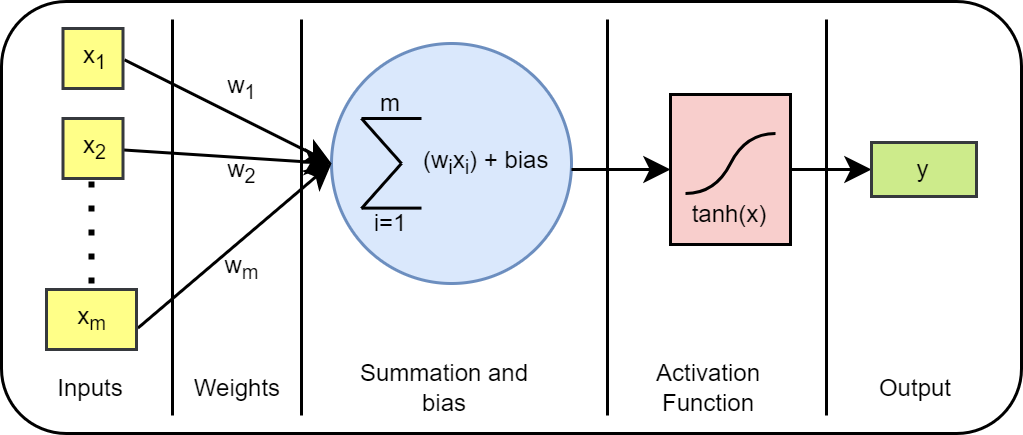
\includegraphics[width=0.95\textwidth]{img/Perceptron.drawio.png}
    \caption{The Perceptron and its components, the input layer, the weights, the weighted sum and bias, the activation function and the output layer.}
    \label{fig:perceptron}
\end{figure*}

To obtain the output of a Perceptron (a prediction), its weights are multiplied by the inputs, then the sum of these multiplications are summed and then a bias is added this result. This weighted sum of the input features can be calculated through Equation \ref{eq:perceptron}. 
\begin{equation}\label{eq:perceptron}
\displaystyle\sum_{i=1} ^{m} (x_i w_i)+bias
\end{equation}
Where $m$ is the number of inputs, $x_i$ and $w_i$ are the inputs and weights and $i$ is the number of the input. Finally, the weighted sum of the input features (and bias) are input through an activation function, which in the original perceptron is a \textit{Step function}, but in Figure \ref{fig:perceptron}, which shows a diagram of the Perceptron structure, is a \textit{Hyperbolic tangent} function. The result of the activation function is the output of the Perceptron.

The learning process of the Perceptron is adjusting the weights and the bias so that the hyperplane can separate the training data up to a set metric.

%While the Perceptron can only solve Linearly separable problems, the Multi Layer Perceptron (MLP) can solve non-Linear problems. 
By stacking layers of multiple Perceptrons, one can approximate any continuous function, rather than only linear functions, thus being able to solve both linear and non-linear problems. MLPs are also known as Fully Connected (FC) neurals networks when combined with other modern neural networks.
The general structure of a Multi Layer Perceptron (MLP), as shown in Figure \cite{fig:mlp-structure} consists on a input layer, one or more hidden layers, and a output layer.

\begin{figure*}[!ht]
    \centering
    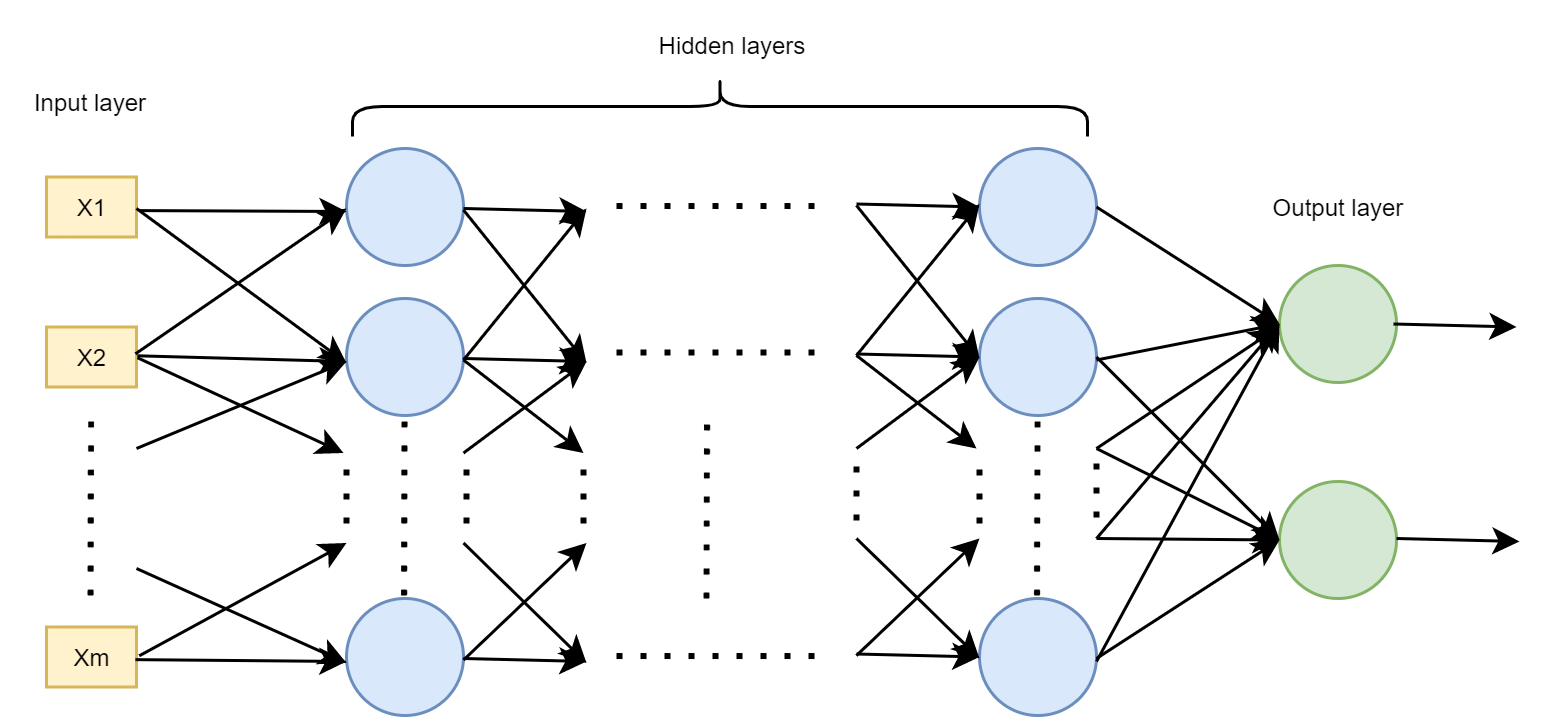
\includegraphics[width=0.95\textwidth]{img/MLP.drawio.png}
    \caption{The Multi Layer Perceptron}
    \label{fig:mlp-structure}
\end{figure*}

The training procedure for the MLP is called \textit{Backpropagation}. It is a process in which the loss value is calculated to measure the error rate of a output. The loss value is used to adjust the weights of the neural network in the reverse sequence of the prediction process. Gurney et. al.\cite{gurney2018introduction} further details the Perceptron and the Multi Layer Perceptron and how the learning on each of them occurs.

When training MLPs, some problems may arise. Overfitting and Underfitting, are, respectively, learning to match the exact pattern of the training data, and not approximating (or learning) the desired pattern enough, in both cases, the network fails to generalize to data outside of the training set. For Overfitting, there are many techniques that mitigate this problem, such as dropout (when some neurons are randomly deactivated when training), and cross validation (split training set in chunks and training with random chunks). Underfitting, on the flip side, may mean that the complexity of the model is too small for the train set or that the training data is insufficient. 
%or learning rate (the size of Backpropagation adjustments)

\section{Convolutional Neural Networks}\label{sec:CNN}


The concept of Neural Networks can also be applied on to computer vision, by combining the concept of convolutions and neural networks, Kunihiko Fukushima created the precursor of modern Convolutional Neural Networks (CNNs), the "neocognitron"\cite{neocognitron1980} in 1980.

To understand CNNs, one must first understand the convolution operation, used in many image processing techniques.
%https://vincmazet.github.io/bip/filtering/convolution.html
\begin{figure*}[!ht]
    \centering
    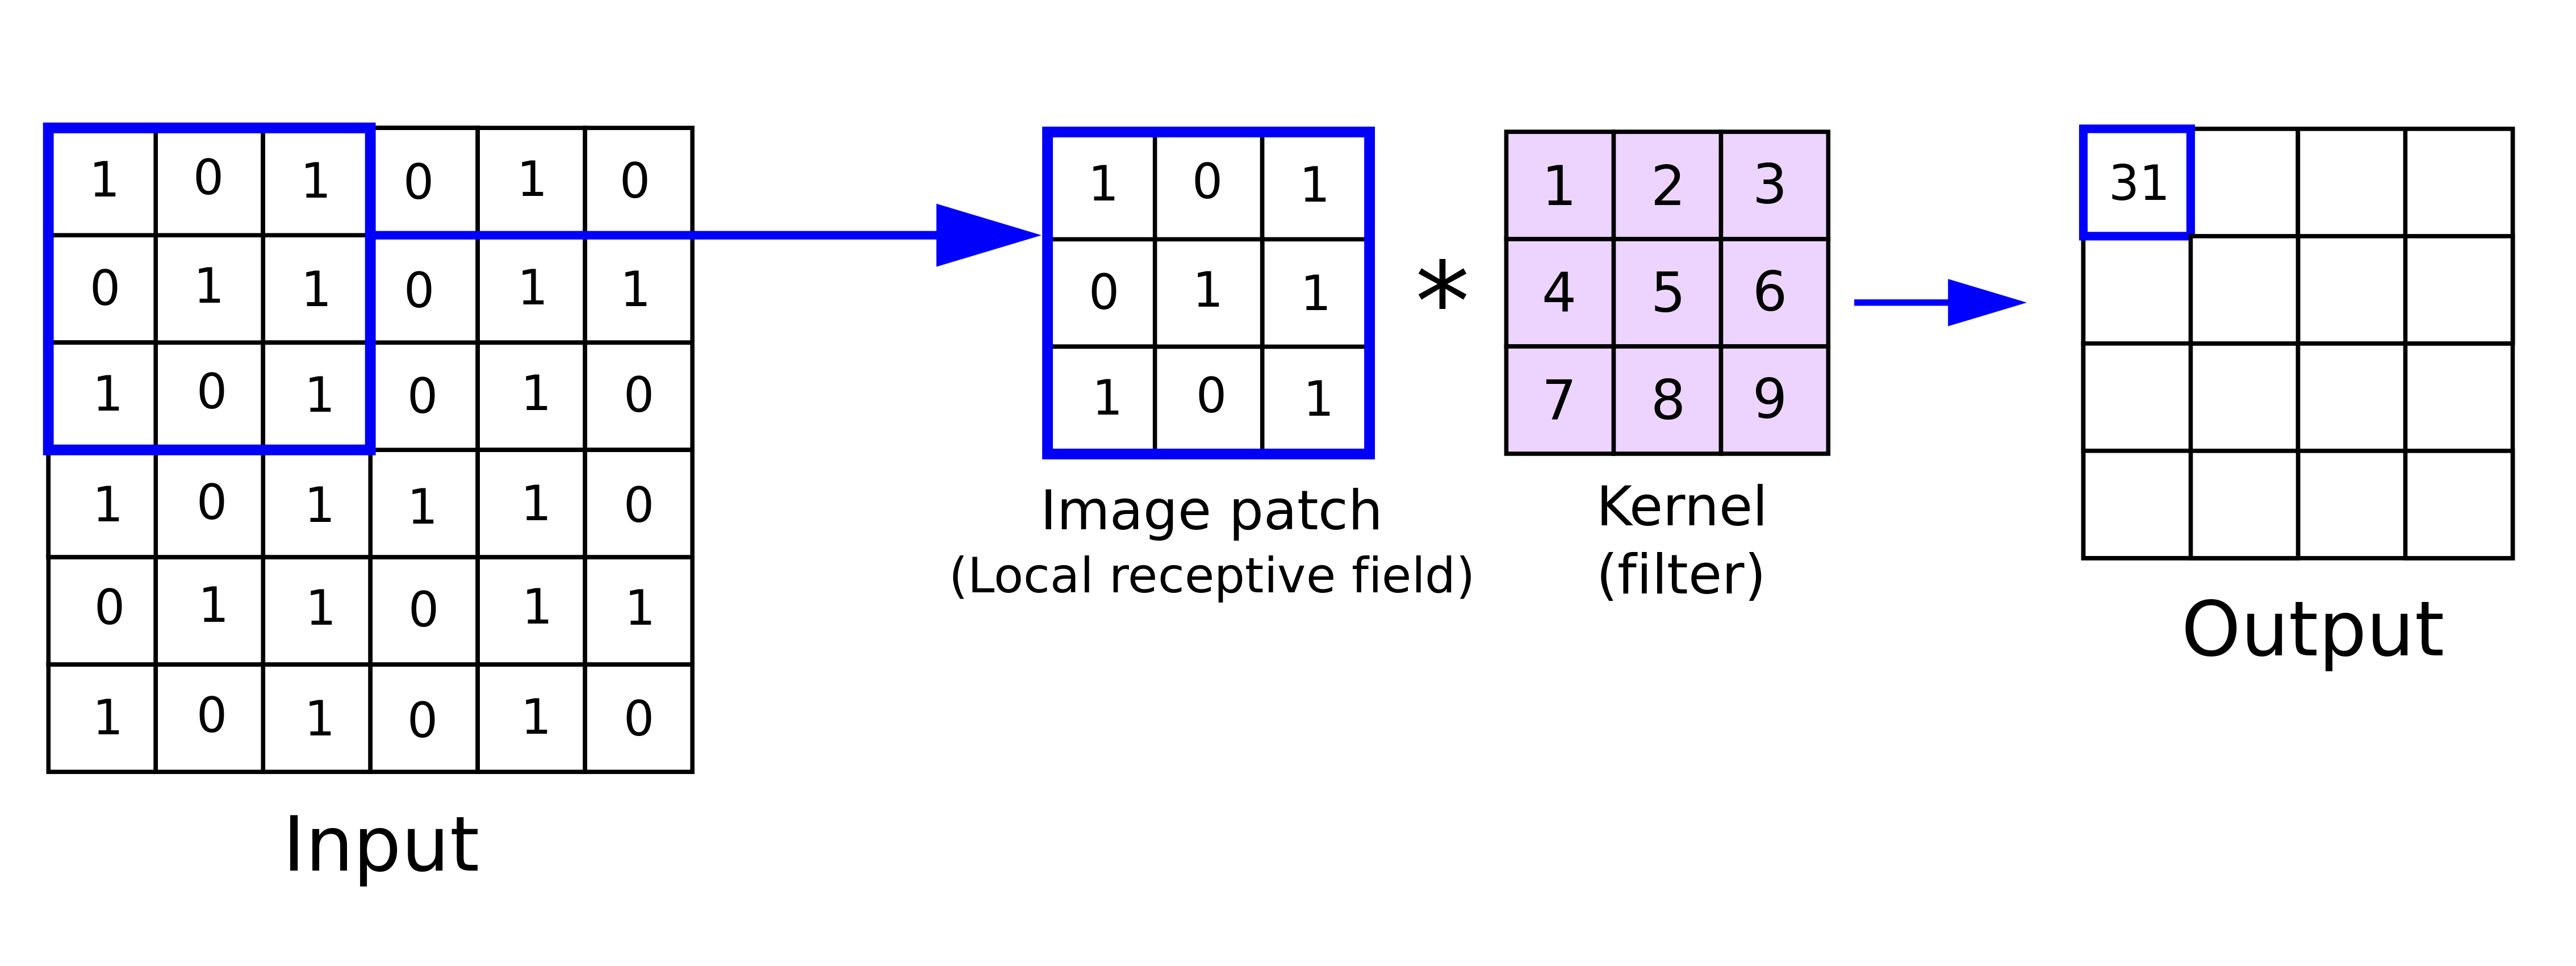
\includegraphics[width=0.95\textwidth]{img/convolution.png}
    \caption[The Convolution Operation]{The Convolution operation, this is the main operation behind Convolutional Neural Networks. Image author: Anh H. Reynolds\footnotemark}
    \label{fig:convolution}
\end{figure*}
%https://anhreynolds.com/blogs/cnn.html

Convolutions consist on applying a filter (or mask), a matrix of values, to a image. As exemplified in Figure \ref{fig:convolution}\footnotetext{\url{https://anhreynolds.com/blogs/cnn.html}}. The operations consists on multiplying each value on the mask for the equivalent pixel (on the current image patch) in the image, then sum all results of these multiplications, this will be the new pixel value of the resulting image/feature map.

%\pva{formula aqui?}

In CNNs, each value of the filter is learned, as if the wheights to be learned in the neural networks are now the values of the convolutional mask.
Each convolution layer has its learned weights for their filters, therefore each convolution layer will process the inputs even further, each layer passing its output to the next.


CNNs also use an operation called Pooling in order to reduce the size of the of the input of a layer (downsample), and consequently speed up computation, by "distilling" the features they become more robust to noise.

The two most common methods of pooling are average and max pooling. Max pooling takes the max value of each neighboring neurons/inputs while average pooling is the average value of each neighboring neurons/inputs. As represented in Figure \ref{fig:avgmax-pooling}.

There are also two different ways to perform Pooling operations. Local pooling reduces the output of the previous neurons/inputs per channel.
Global pooling combines values of previous neurons/inputs across dimensions, or channels, in the feature map. 

%https://androidkt.com/explain-pooling-layers-max-pooling-average-pooling-global-average-pooling-and-global-max-pooling/
\begin{figure*}[!ht]
    \centering
    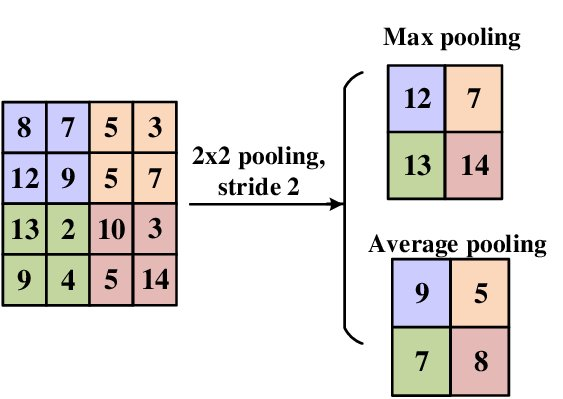
\includegraphics[width=0.55\textwidth]{img/pooling.jpg}
    \caption{Local Max and Average Pooling representation. Image authors are Yingge et. al.\cite{yingge2020pooling}}
    \label{fig:avgmax-pooling}
\end{figure*}

In the first stage of a traditional image classification CNN is comprised of convolutional and pooling layers, extracting and disitlling characthistics as the layers get deeper into the model, this is called the feature extraction stage. Then, the features are input to the classification stage, which is usually a fully connected layer of neurons (a Multilayer Perceptron). The classification stage outputs 
%the activations or probabilities for each class, which then are used to decide 
the predicted class. This generic image classification CNN is shown in Figure \ref{fig:generic-cnn}.
%in the 1980s by Yann LeCun, a postdoctoral computer science researcher.
\begin{figure*}[!ht]
    \centering
    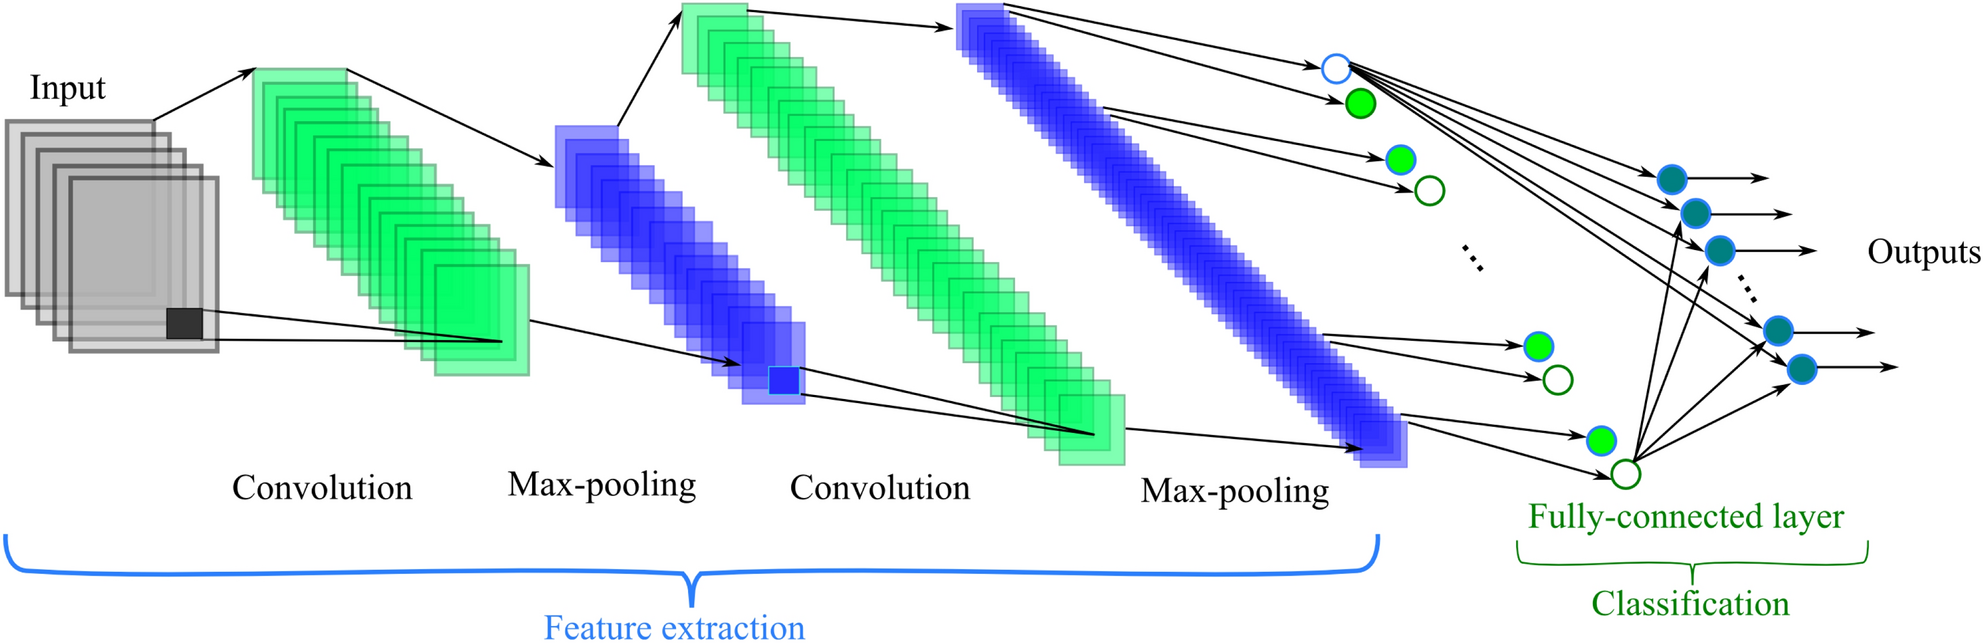
\includegraphics[width=0.95\textwidth]{img/generic-convnet.png}
    \caption{A generic image classification CNN architecture, representing the feature extraction stage and the classification stage. Note that as the inputs progress through the CNN the width and height of the inputs become smaller, but the number of feature channels/dimensions increases. Image authors are Khozeimeh et. al.\cite{khozeimeh2021cnnimage}}
    \label{fig:generic-cnn}
\end{figure*}

As convolutional layers get deeper, the level of abstraction also gets higher, as an example, in a generic image classification CNN, the last layers the features may represent more abstract concepts, such as the presence of objects and complex shapes such as cars. These abstractions depend on what images the CNN was trained and what is it supposed to classify. 

Once a CNN is trained with success, it should have learned representations as features that allow it to differentiate between classes. By training a new classifier on the already existent learned concepts (features) in the last convolutional layers, one can modify this generic CNN to classify between dogs and cats or types of car. One could also use the same trained generic CNN and continue training it on a different task, using the already learned concepts as a head start, the CNN would also learn more specific concepts to this task as the training continues. This is called transfer learning. 

%2009
One of the most popular datasets and challenges for CNNs is the The ImageNet Large Scale Visual Recognition Challenge (ILSVRC)\footnote{\url{http://www.image-net.org/}}\cite{deng2009imagenet}, in 2012 it hosted the work that ushered a boom in CNN research and development when AlexNet achieved a top-5 error of 15.3\% in the ILSVRC, more than 10.8 percentage points lower than that of the second place. The ImageNet dataset has more than 100.000 "synonym sets" which are sets of words or phrases that represent the image. The dataset holds multiple challenges for tasks such as Image classification, Single-object localization and Object detection, each of the subsets for these tasks have 1000 classes (or objects).

A CNN trained on the ImageNet dataset, can learn a wide variety of abstractions, from cars to dogs, because of the wide scope of their image classification task. This makes CNNs pre-trained in the ImageNet dataset specially performant as transfer learning models~\cite{huh2016makes}.

With the success of CNNs, researchers started modifying and applying these models on other domains, such as audio, time series and natural processing language

The equivalent of the ImageNet dataset for the audio classification is the Audioset\footnote{\url{https://research.google.com/audioset/}}~\cite{gemmeke2017audioset}. It is an ontology of 632 audio classes and 2,084,320 human-labeled 10-second sound clips collected from YouTube videos. Its classes range from human and animal sounds, musical instruments and genres, and common everyday environmental sounds.

With the advent of deeper CNNs, one problem also surfaced: The vanishing gradient problem, it occurs when the error propagation makes the training diverge, the values of weights become too small. To avoid this problem, there are multiple techniques, such as the Rectified Linear Unit (ReLU) activation function~\cite{krizhevsky2012relu}, and lower the learning rate, thus taking smaller steps when adjusting the weights.

\section{The VGG Convolutional Neural Network}\label{sec:VGGish}

The VGG Convolutional Neural Network~\cite{simonyan2014VGG} was designed for the ImageNet Challenge in 2014, where it won the first and second place in localization and classification tasks. It's input is a 224$\times$224 RGB image. The main contribution of this network is that is showed that even with a very small receptive field (3$\times$3, which is the smallest size to capture the notion of left/right, up/down and center, by increasing the depth of a network, it could still outperform all other CNN based methods at the time.

This architecture has 6 configurations with different depths that are connected to two Fully Connected (FC) layers, two of 4096 channels and a final one with a 1000 channels (The Image Net challenge had a 1000 classes), followed by a soft-max layer that outputs the predicted class.
The configuration of the fully connected layers is the same in all configurations. All hidden layers used rectification (ReLU)~\cite{krizhevsky2012relu} non-linearity. Figure \ref{fig:vgg16} shows the most popular variation, the VGG-16 (Configuration D) and its layers, as described above.

\begin{figure*}[!ht]
    \centering
    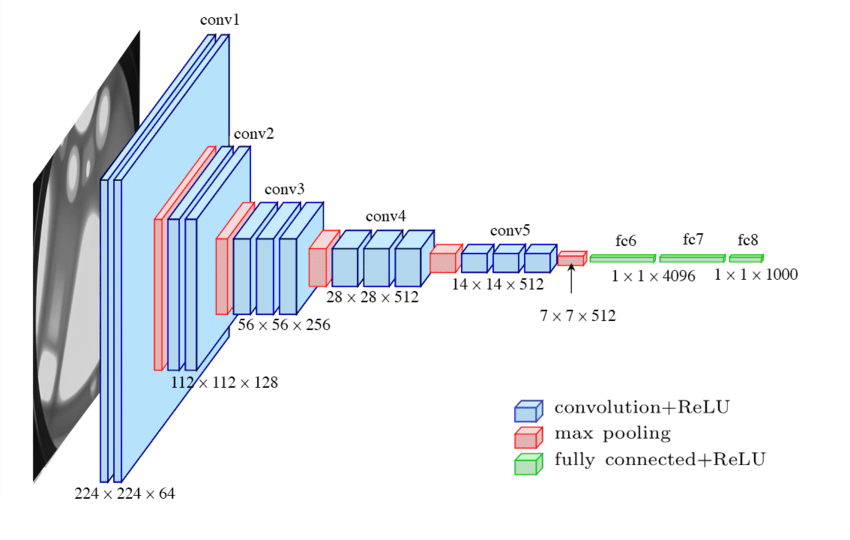
\includegraphics[width=0.95\textwidth]{img/vgg16.png}
    \caption{VGG-16 architecture, image authors are Ferguson et. al.\cite{ferguson2017vggimage}.}
    \label{fig:vgg16}
\end{figure*}

\section{VGGish}\label{sec:VGGish}
The VGGish is a variation of the VGG-11 (Configuration A), created by the authors of the YouTube8m dataset ~\cite{abu2016youtube}, with some modifications to perform audio (spectogram) classification and embeddings generation).

Specifically, the input size was modified to 96$\times$64 for log mel spectogram audio inputs. The last group of convolution and maxpool layers were removed. In order to created a compact embedding layer, the 1000 channels wide FC layer at the end was changed to a 128-wide FC layer. This final layer does not have an non-linear activation.

\section{The Inception Convolutional Neural Network}\label{sec:Inception}

The Inception Convolutional Neural Network or GoogLeNet, ~\cite{szegedy2015Inception} was designed for the ImageNet Large-Scale Visual Recognition Challenge in 2014, it features many techniques in order to increase efficiency of deep CNNS.

In order to achieve this increased efficiency, the authors created a module to capture as much information as possible, both in local and global context, by using multiple kernel sizes in the same convolutional layer. To optimize for computational cost and speed, the creators also avoided naively stacking layers, for it is computationally expensive.

The solution proposed by the authors of the inception CNN is to use compute multiple filters in the same level, with varying convolutional filter sizes.

The ``Naive'' inception module, as shown in Figure \ref{fig:naive-inception} consists on a convolutional layer using 3 different filter sizes, 1$\times$1, 3$\times$3 and 5$\times$5. Along with a max pooling operation. The outputs are then concatenated by the end of the inception module.

\begin{figure*}[!ht]
    \centering
    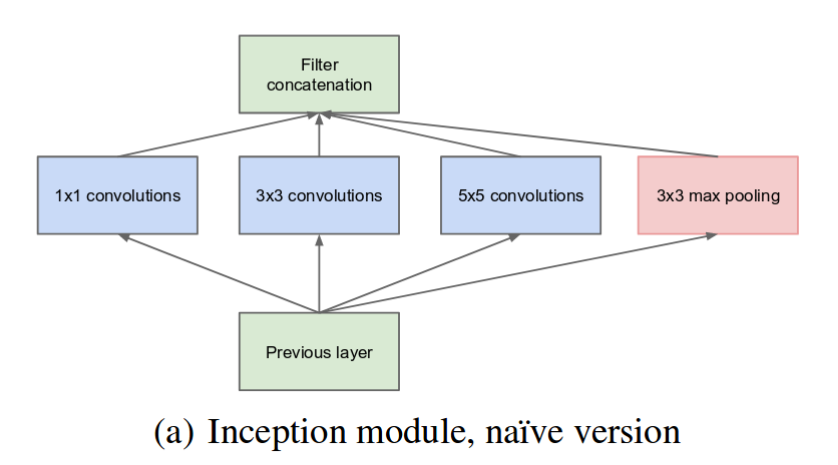
\includegraphics[width=0.95\textwidth]{img/naive-inception.png}
    \caption{The ``Naive'' inception module, image authors are Szegedy et. al.~\cite{szegedy2015Inception}.}
    \label{fig:naive-inception}
\end{figure*}

% \begin{figure*}[!ht]
%     \centering
%     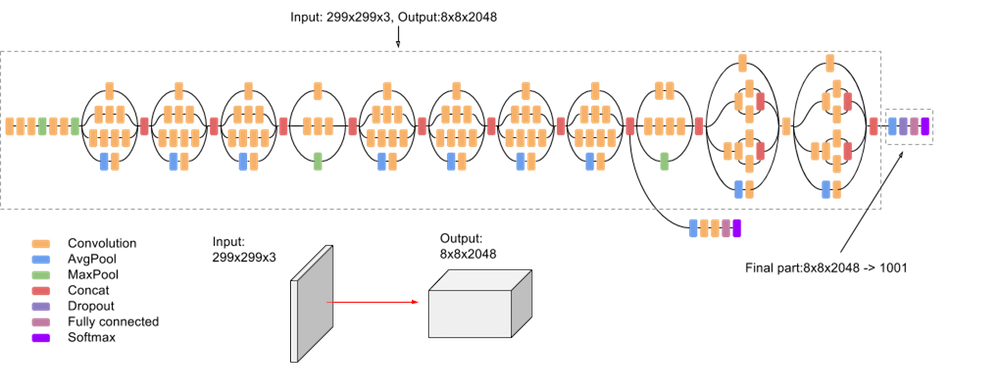
\includegraphics[width=0.95\textwidth]{img/inceptionv3.png}
%     \caption{Inception V3 Architecture\footnote{\url{https://cloud.google.com/tpu/docs/inception-v3-advanced}}.}
%     \label{fig:naive-inception}
% \end{figure*}

In order to reduce computational costs further, the authors added 1$\times$1 convolutions after the max pooling step and before the 3$\times$3 and 5$\times$5 convolutions. By doing this the authors reduce the amount of processing done by reducing the quantity of input channels before the convolutions. This improvement was named ``The inception module with dimension reduction'' and it is represented in Figure \ref{fig:red-dim-inception}.  

\begin{figure*}[!ht]
    \centering
    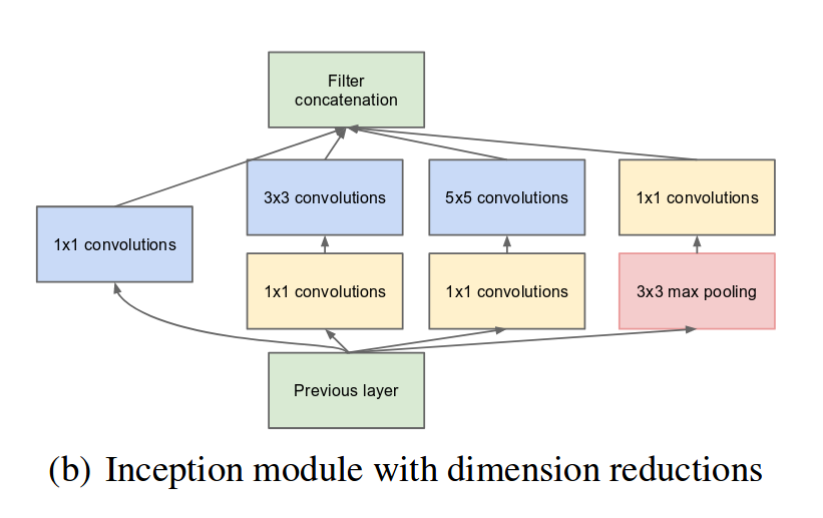
\includegraphics[width=0.95\textwidth]{img/inception-module.png}
    \caption{The inception module with dimensional reduction, image authors are Szegedy et. al.~\cite{szegedy2015Inception}.}
    \label{fig:red-dim-inception}
\end{figure*}

By stacking 9 inception modules with dimension reduction and using 2 intermediate classifiers, essentially computing prediction values and using these values to compute auxiliary losses, which are then used to compose the final loss in the training process in order to avoid the vanishing gradient problem.

As shown in Figure \ref{fig:inception-architecture} It is still deeper (it has 22 convolutional layers) than the deepest VGG configuration (with 19 convolutional layers).

\begin{figure*}[!ht]
    \centering
    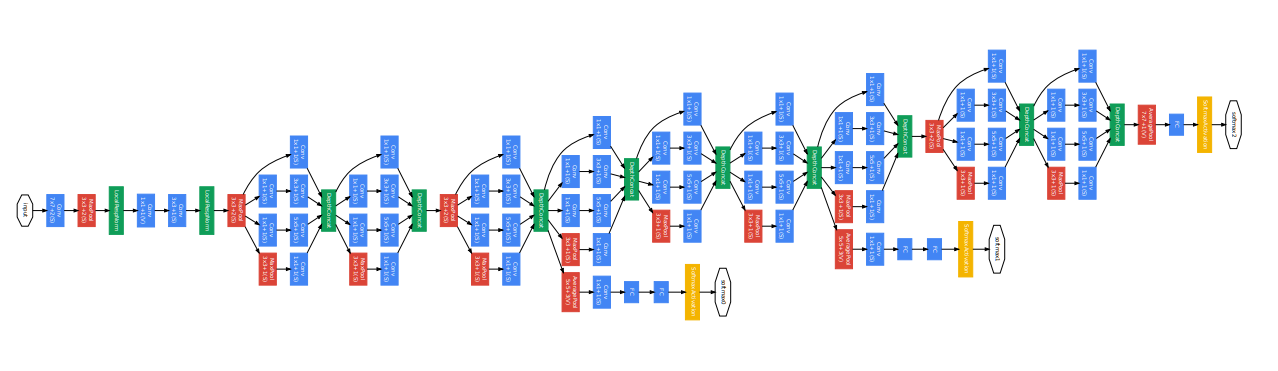
\includegraphics[width=0.95\textwidth]{img/inception-architecture.png}
    \caption{The complete inception convolutional neural network, image authors are Szegedy et. al.~\cite{szegedy2015Inception}.}
    \label{fig:inception-architecture}
\end{figure*}

InceptionV2 and InceptionV3 networks~\cite{szegedy2016rethinking}
For the inceptionV2 computational efficiency was improved by factorizing the convolutions, convolutions with 5$\times$5 size kernels were factorized into two 3$\times$3 sequential convolutions, this improves computability (because 3$\times$3 convolutions use 2.78 times less operations than 5$\times$5) while actually improving performance. They also factorized the 3$\times$3 convolutions into one 1$\times$3 and 1$\times$3 convolutions. These factorized convolutions are performed on the same input to avoid excessive dimension reduction (information loss).

The InceptionV3 CNN used all the upgrades of the InceptionV2, and improved performance further by incorporating the RMSProp Optimizer \cite{tieleman2017rmsprop}, factorized 7$\times$7 convolutions ( 1$\times$7 convolutions followed
by 7$\times$1 convolutions.), batch normalization in the Auxillary Classifiers, and Label Smoothing (It is a modification in the loss function that prevents the network having high confidence in a class) for preventing overfitting.


% RMSProp Optimizer.
% Factorized 7x7 convolutions.
% BatchNorm in the Auxillary Classifiers.
% Label Smoothing (A type of regularizing component added to the loss formula that prevents the network from becoming too confident about a class. Prevents over fitting).

The Inception CNNs continued to improve further with InceptionV4 and Inception-ResNet ~\cite{szegedy2017inceptionv4}, but we will not detail them here for they are not used in the scope of this work.



\section{Feature Fusion}
\label{sec:feature_fusion}

Since we are using information from two different domains, image and audio, it is also important to think how one can fuse information from both these domains without . 
Which method is best to fuse the information from these different domains.

Snoek et al. \cite{snoek2005featurefusion} presents two main strategies for information fusion in semantic video analysis: 
\begin{itemize}
    \item \emph{Early fusion} methods (Figure \ref{fig:early-fusion}), which works directly with the extracted features.
    \item \emph{Late fusion} methods (Figure \ref{fig:late-fusion}), which operates on classification outputs from specialized models.
\end{itemize}

% late fusion comes at cost of training time
In the work by Snoek et. al.\cite{snoek2005featurefusion}, the Late fusion approach tends to give better performance on most semantic concepts (multilabel video classification) at the cost of increased computability costs. However, the authors also conclude that the late and early fusion approaches should be compared are per concept (in a multilabel situation).%, which one can generalize to per task in binary tasks.

\begin{figure*}[!ht]
    \centering
    \begin{subfigure}[b]{0.55\textwidth}
        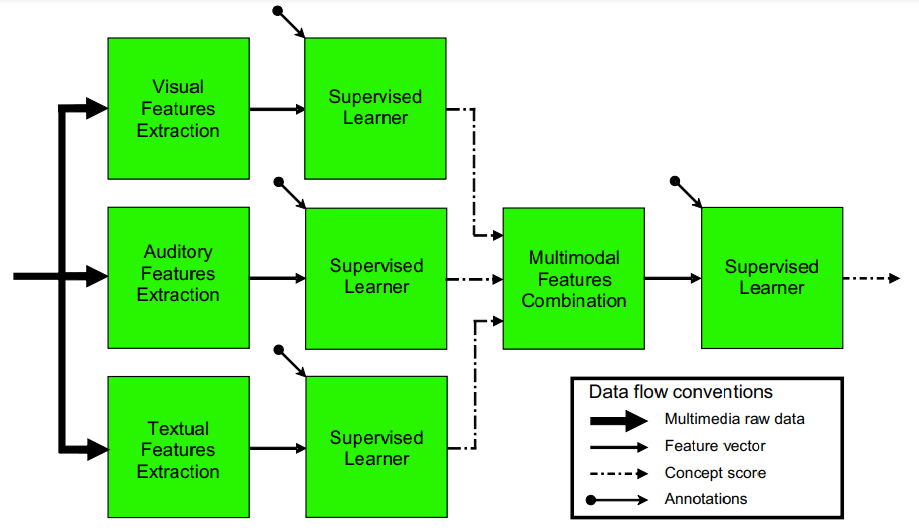
\includegraphics[width=0.94\textwidth]{img/late-fusion.png}
        \caption{The late fusion approach, in it there is a machine learning model for each unimodal feature and a final model to fuse the outputs of each unimodal model.}
        \label{fig:early-fusion}
    \end{subfigure}
    \begin{subfigure}[b]{0.44\textwidth}
        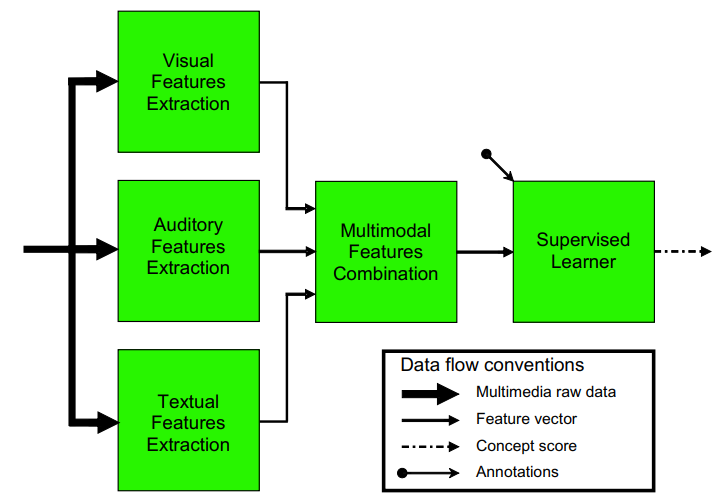
\includegraphics[width=0.94\textwidth]{img/early-fusion.png}
        \caption{The early fusion approach, it uses a single multimodal machine learning model to both aggregate and classify all features.}
        \label{fig:late-fusion}
    \end{subfigure}
    \caption{The late and early fusion methods for feature fusion. Image authors are Snoek et. al.~\cite{snoek2005featurefusion}.}
\end{figure*}

\section{Method and experimentation}
\label{sec:method}
In this section we detail our method for sensitive content detection in video. We split our approach into three parts: feature extraction, feature fusion and feature classification, as illustrated in Figure \ref{fig:model}.
\begin{figure*}[!ht]
    \centering
    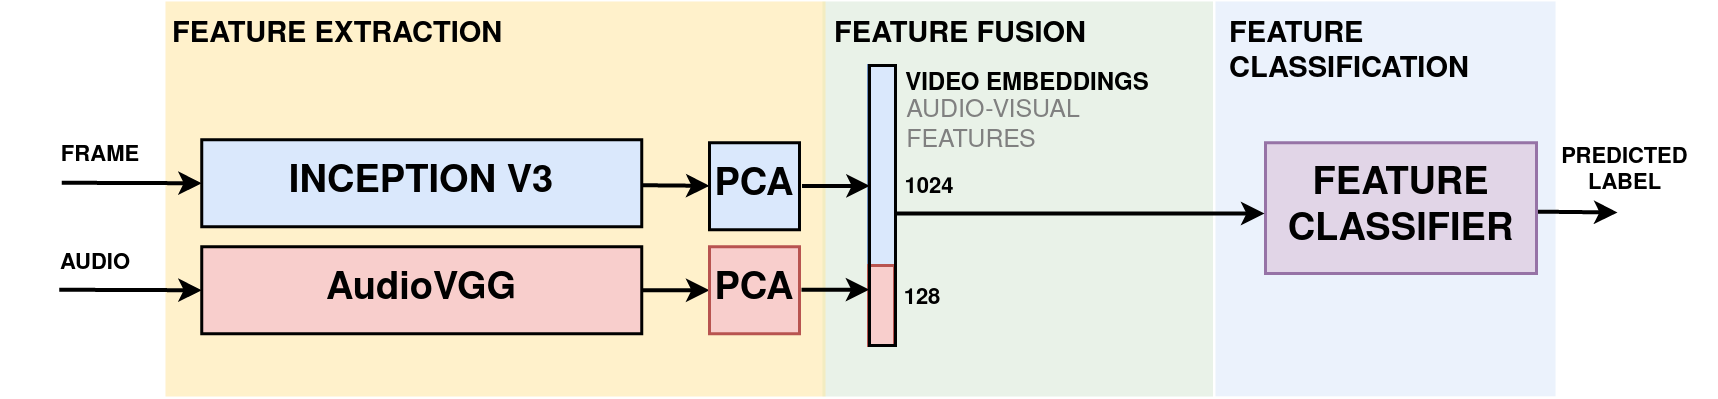
\includegraphics[width=0.9\textwidth]{img/model-2.png}
    \caption{Bimodal architecture for NSFW video classification.}
    \label{fig:model}
    \vspace{-1em}
\end{figure*}

In the feature extraction stage, firstly we split the frames and audio from the video; then, for each media, we use a CNN to extract the features (or embeddings) from each simultaneous video segment. In the second stage, Feature Fusion, we concatenate both audio and frame features. If the classification model is not sequential, we also aggregate the features in this stage. Finally, in the feature classification stage we feed one of the classification models to be experimented with.

\subsection{Video Embeddings Extraction}
\label{subsec:video_features}

CNNs tend to learn low-level features (\textit{e.g.}, in the visual domain: edges, corners, contours) at their first layers. At the intermediate and final layers, the combination of these features helps to extract more complex features, resulting in a vector of continuous values, referred to as \textit{embeddings}, that might be used for classification and other tasks. In this work, we use two benchmark CNNs to extract both image and audio \textit{embeddings} by using a transfer learning technique~\cite{tan2018survey}.



%Afterwards, we apply PCA (+ whitening) to reduce feature dimensions to 1024, followed by quantization (1 byte per coefficient).
%These two compression techniques reduce the size of the data by a factor of 8. The mean vector and covariance matrix for PCA was computed on all frames from the Train partition. We quantize each 32-bit float into 256 distinct values (8 bits) using optimally computed (non-uniform) quantization bin boundaries. We confirmed that the size reduction does not significantly hurt the evaluation metrics. In fact, training all baselines on the full-size data (8 times larger than what we publish), increases all evaluation metrics by less than 1%.

\todo{explicar pq escolheu as cnns (youtube) e qual foram os paramretros usados (pca e hiperparametros)}
By using the feature extraction method created for the Youtube-8m benchmark, we can test an feature extraction method that is powerful enough to represent features that can be in multiple tasks, such as multi-label video classification, video recommendation, and human activity recognition.

"Since the video-level representations are unsupervised (extracted independently of the labels), these representations are far less specialized to the labels associated with the current dataset, and can generalize better to new tasks or video domains."~\cite{abu2016youtube}

In order to validate our dataset, we used the same feature extraction method used in the Youtube-8m dataset challenges~\cite{abu2016youtube}, both networks were pre-trained and frozen and they were not retrained for application sensitive content classification. Which gives future works an opportunity to develop even more efficient and smaller feature extraction networks for this specific task.


To generate image frame features and audio features we decode each video at approximately 1 frame-per-second and feed an InceptionV3  network~\cite{szegedy2016rethinking} pre-trained on the ImageNet\footnote{\url{http://www.image-net.org/}} dataset.
 
We also make use of a AudioVGG~\cite{hershey2017cnn} network with pre-trained weights in the Audioset\footnote{\url{https://research.google.com/audioset/}} dataset to extract the audio embeddings. Each of these CNNs were used as published by their authors; the only modification was the removal of classification layers in both CNNs to obtain their respective embeddings.

Next, we apply Principal Component Analysis (PCA)~\cite{wold1987principal} to each of the outputs to reduce the dimensions of both embeddings and to generate feature vectors of size 1024 and 128 for frame and audio embeddings respectively.
%DETALHAR MAIS AQUI DE QTO PRA QTO O PCA REDUZ

\subsection{Feature Fusion}
\label{subsec:feature_fusion}

Once we have the features from both image and audio, we should make a decision about which method is best to fuse the information from these different domains. Snoek et al. \cite{snoek2005featurefusion} presents two main strategies for information fusion in semantic video analysis: \emph{Early fusion} methods, which works directly with the extracted features, and \emph{Late fusion} methods, which operates on classification outputs from specialized models.
%\todo{For a more recent survey about data fusion and multimedia retrieval, please refer to \cite{jiang2013features}.}
In this work, because we have high abstraction level features, we opted to investigate the most simple approach, which is to use a single model on the concatenated features from both media inputs.

Specifically, we concatenate both image and audio embeddings extracted in the current frame and audio window in order to compose the final embeddings as a sequence of the same size of the number of seconds of the video. After this concatenation, each time-step has 1,152 features: 128 audio features and 1024 frame features.

Notice that with this approach, the video is transformed into a time series, and to use it in non-sequential models (\textit{e.g.}~SVM, KNN, and MLP) we need to turn this sequence into a single feature vector that represents the whole video. In our setting, we did that by taking the average, median, standard deviation, min, and max values for each feature to represent the entire video. In summary, we turn the sequence of features with size $n$ and shape $n$ by 1,152 into a single feature with shape 1 by 5,760.

\subsection{Classifiers}
\label{subsec:classifiers}

% \todo[inline]{porque foi escolhidos esses modelos de classficação, qual a relação deles com o nosso tipo de dado de vídeo.}

For the feature classification task, we will investigate both sequential models (which use the extracted embeddings in a time series format), and non-sequential ones (which use a single aggregated embeddings vector).
We want to experiment with both approaches in order to investigate if a more compact format, such as the single embeddings vector, can yield results at least as good (or even better) than the full feature sequence data.
%Furthermore, we can test if a sequential model can outperform a non-sequential model in specific cases that demand long term memory, such as long videos with very small sensitive scenes.
As an example, one can think of a long video that has a pornographic scene in one second out of its entirety. 
In a non-sequential representation of the extracted features, this short pornographic fragment could be left ``hidden'' among the other non-pornographic frames of the video, as illustrated in Figure \ref{fig:model-non-sequence}.
\begin{figure*}[!ht]
    \centering
    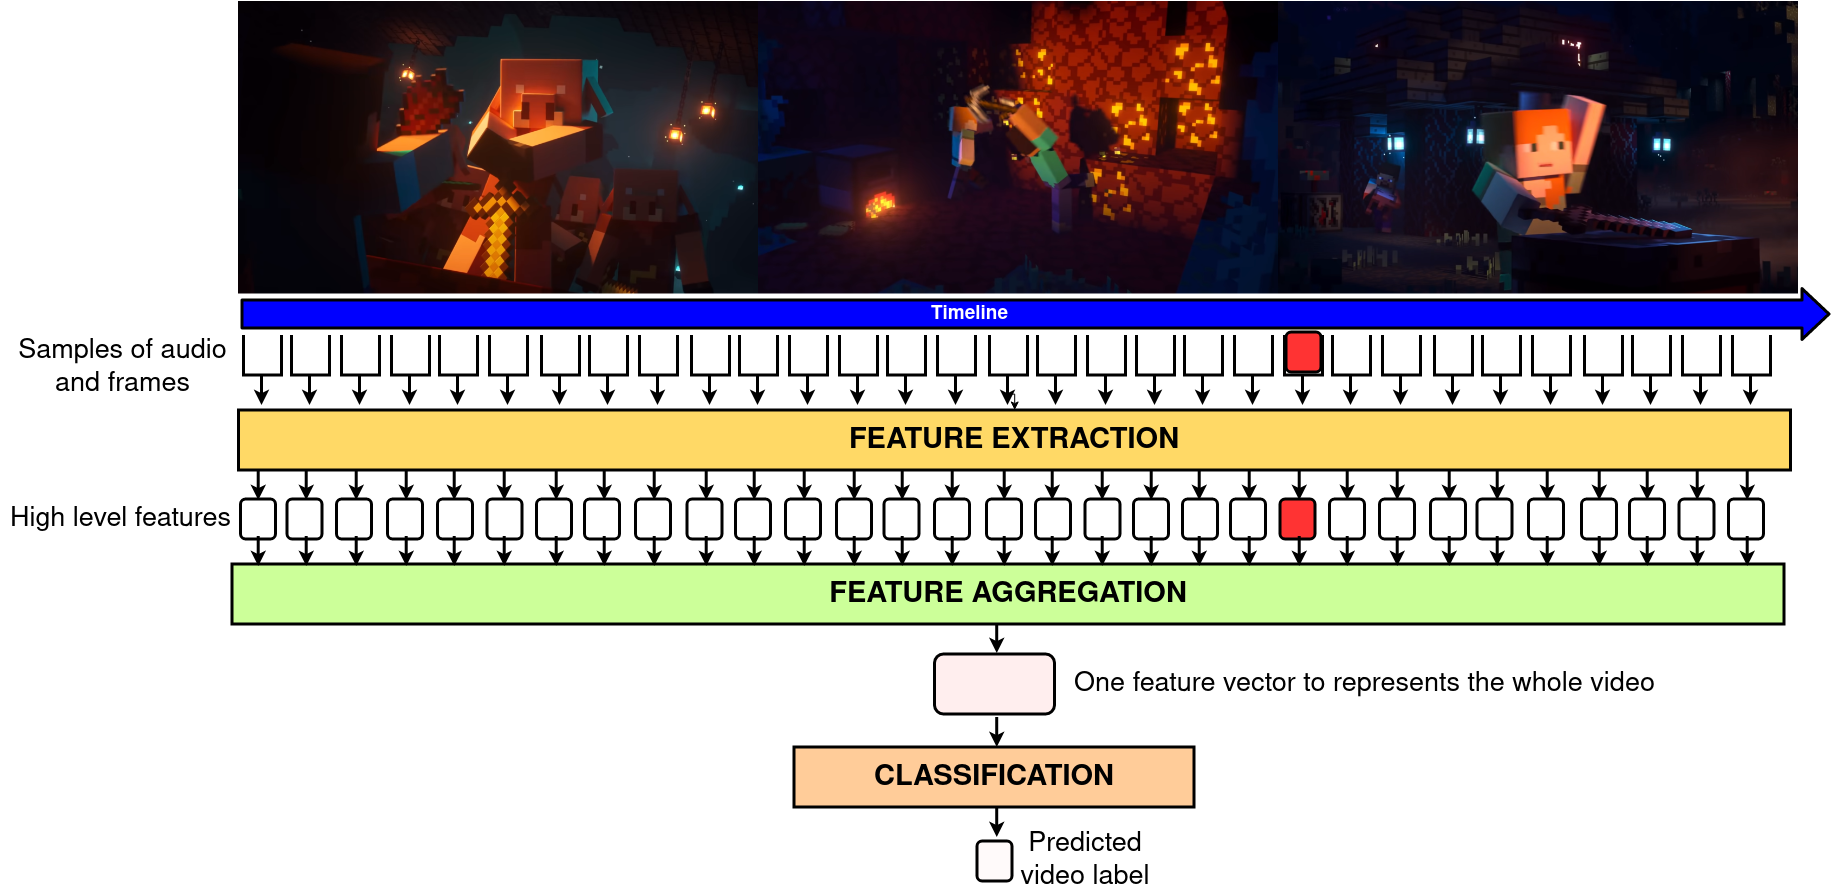
\includegraphics[width=0.9\textwidth]{img/model-non-sequence.png}
    \caption{Sequential features with aggregation, the sensitive scene (red) might vanish among the the other scenes during aggregation.}
    \label{fig:model-non-sequence}
    \vspace{-1em}
\end{figure*}
In a sequential representation, although time series classifiers usually output a prediction after reading the entire sequence, the embedding vectors of each second of the video would not be aggregated and thus could be analysed section by section, as illustrated in Figure \ref{fig:model-sequence}.

\begin{figure*}[!ht]
    \centering
    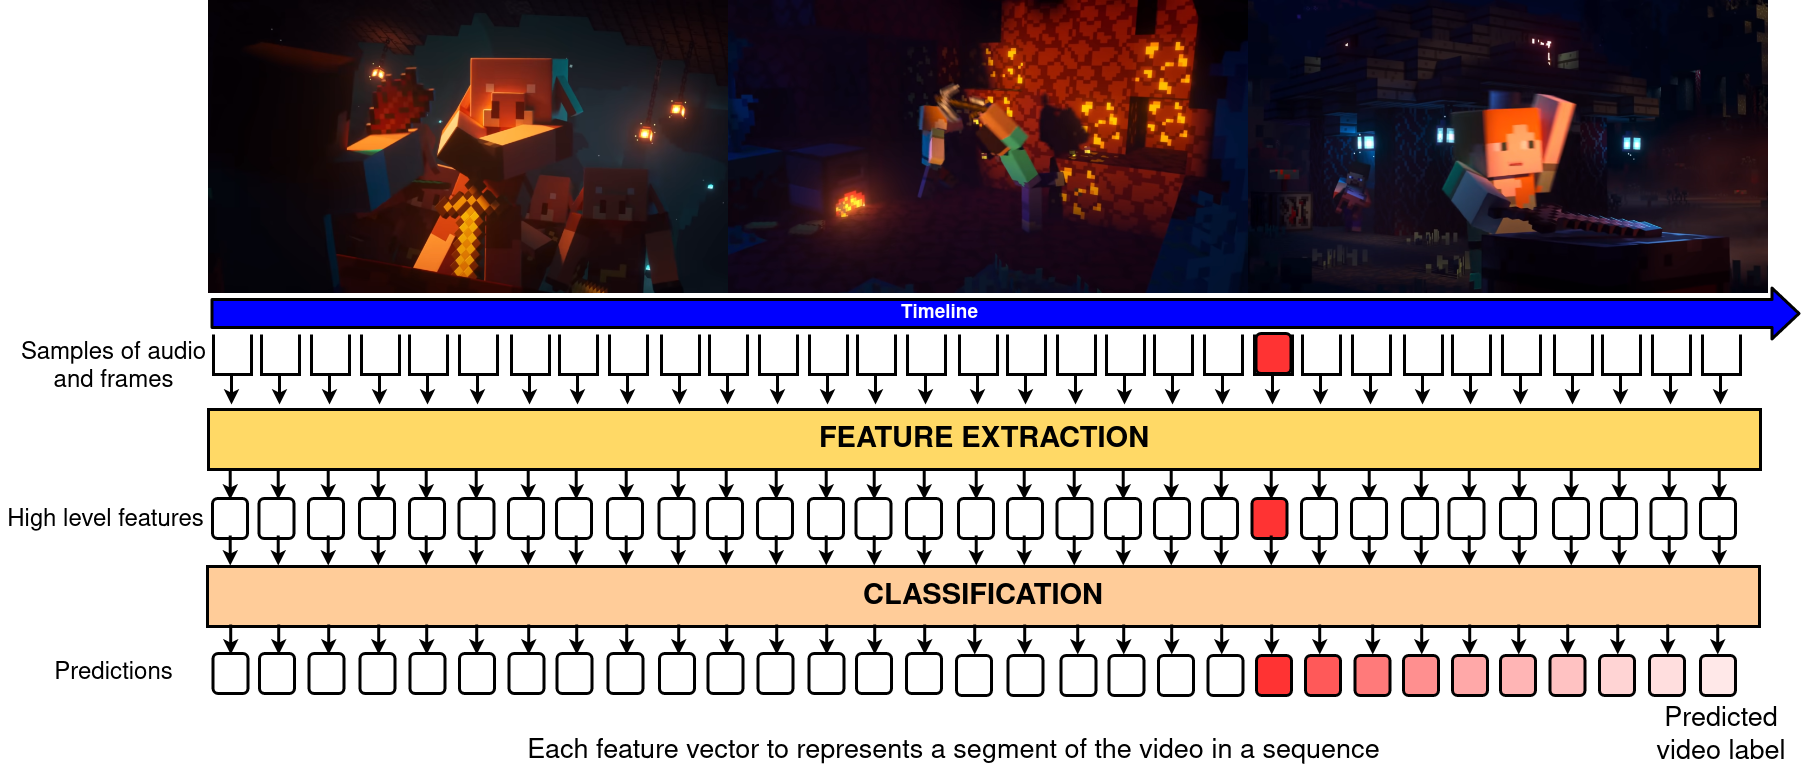
\includegraphics[width=0.9\textwidth]{img/model-sequence.png}
    \caption{Sequential features with no aggregation. In a output after reading the entire sequence, this can also be susceptible to information vanishing.}
    \label{fig:model-sequence}
    \vspace{-1em}
\end{figure*}
Although a sequential representation contains possibly much more redundant data than the non-sequential one, it could give the sequential classification model an important edge of detail over the less granular non-sequential ones.
% To do the feature classification task, we experimented four well known classification mohave dels, one using extracted video features in the time series format, and three that use a single aggregated feature vector.

For the sequential classification model, we chose the Long Short-Term Memory (LSTM)\cite{hochreiter1997long} networks.
It has been a commonly used time series classification baseline model. %\todo{mayber say we'll test GRUs?}

For the non-sequence models, we chose Support Vector Machines (SVM)~\cite{cortes1995support}, K-Nearest Neighbors (KNN)~\cite{peterson2009k}, and Multilayer Perceptron (MLP)~\cite{haykin2009neural}.
Among all of the experimented models, the \textit{Support Vector Machine (SVM)} is the most used in the literature.
% \begin{enumerate}[leftmargin=*]
% \item 
It is a classification model in which the data is mapped into a higher dimension input space, where an optimal separating hyper-plane is constructed.
% These decision surfaces are found by solving a linearly constrained quadratic programming problem.
% \item 
The second model, \textit{K-Nearest Neighbors (KNN)} uses distance measure between training samples so that the k-nearest neighbors always belong to the same class, while samples from different classes are separated by a large margin. 
It was chosen because it used also by related work, although it is a simple classification method.
% \item 
The third model is the \textit{Multilayer-perceptron (MLP)}, which contains layers of nodes: an input layer, an output layer and various hidden layers in between. 
This one was selected because it is also commonly used as a final classifier on deep neural networks.  
% The number of layers used is problem dependent, as is the number of nodes in each hidden layer.
% The weights are adjusted by local optimization using a set of feature vectors so that the network produces the optimal expected output.
% \item 
%Lastly, \textit{Long short-term memory (LSTM)}, different than the feed-forward neural networks, process the entire sequences of data using feedback connections.
% \end{enumerate}

In next the Section, we present the \textit{dataset} created to train and evaluate these classification models.

\section{Dataset}\label{sec:dataset}
% Falar do sampling inicial, da presentatividade dos sets
% falar do balanceamento e do sampling do conjunto de teste
% Falar das talbeas no texto
% colocar o resto das tabelas talvez no appendix
% estatisticas depois de dropar os maiores e os menores videos, sem balanceamento
% usamos o balanceamento dropando apesa porn videos pq os gore sao poucos
% iremos distribuir o dataset na versao balanceada e sem balanceamento
% Comparar nossas escolhas de corte de tempo com o do yt 
% Checked for duplicates by name and size and by fdupes, sem garantias de de não ter subvideos


% Before clipping video based on duration
% Mean:  0:06:18.929511  STD:  0:12:18.237458
% There are 1355 (1.05%) videos longer than 00:30:56
% There are 116 (0.09%) videos shorter than 00:00:05

% Videos:
% Total dataset: 127075
% Total size of videos (calculated individually): 3.5TiB
% Total duration of videos (calculated indiviadually): 11806:21:13
% Improper videos: 67424
% Total size of videos (calculated individually): 1.2TiB
% Total duration of videos (calculated indiviadually): 6953:27:41
% Proper videos: 59651
% Total size of videos (calculated individually): 2.2TiB
% Total duration of videos (calculated indiviadually): 4852:53:31
% Total size of features: '896.3GiB'

% Hot much detail do we go on about the dataset's subclasses? (subclasses por porn and yt, no subclasses on gore)

Our \textit{dataset} is structured into two main classes: videos containing ``safe'' content and videos containing sensitive content.
It is divided into 59,651 safe videos and 67,424 videos with sensitive content.

\begin{table}
\centering
\label{tab:general-stats}
\caption{General statistics of the two main classes of the dataset, tag coverage refers to main tag annotation existence (videos may also have sub tags but no main tag).}
\begin{tabular}{c|r|r} 
\multicolumn{1}{l|}{} & Sensitive  & Safe        \\ 
\hline
Video Count           & 67424      & 59651       \\ 
\hline
Total Duration        & 6953:27:41 & 4852:53:31  \\ 
\hline
Mean Duration         & 00:06:11   & 00:04:52    \\ 
\hline
STD Duration          & 00:04:12   & 00:03:26    \\ 
\hline
Max Duration          & 00:30:55   & 00:30:55    \\ 
\hline
Min Duration          & 00:00:05   & 00:00:05    \\ 
\hline
Total Size            & 1.2TiB     & 2.2TiB      \\ 
\hline
Mean Size             & 19.3MiB    & 39.0MiB     \\ 
\hline
STD Size              & 35.4MiB    & 42.3MiB     \\ 
\hline
Features Size         & 519.4GiB   & 376.8GiB    \\ 
\hline
Tag coverage          & 65392      & 51011       \\ 
\hline
Tag coverage (\%)     & 96,9862    & 85,5157     \\
\end{tabular}
\end{table}
% \subsection{SFW Videos}\label{sec:safe_videos}

For \textit{safe content}, we extracted 50,988 videos from Youtube8M\footnote{\url{https://research.google.com/youtube8m}}~\cite{abu2016youtube}. We chose this dataset because of the size of the dataset (8 million videos) and because of the wide variety of video classification challenges it supports.

We also included 8,663 videos collected from Youtube, hereby refered as cherry-picked, those videos were selected for the purpose of incremeting the amount of "hard" videos, which are videos that could possibly be misclassified as sensitive, such as MMA, breastfeeding, pool party, beach and other videos that have a higher amount of skin exposure. The amount of cherry-picked videos collected are listed by its query in Table \ref{tab:non-yt-count}. The collection was made by automated means, an script automatically searches and downloads all videos from the first 100 result pages.
% One of the objectives of the project is to evaluate the presence of inappropriate videos in educational video repositories. Therefore, in selecting your own videos within YouTube8M, we have chosen videos from \ "Jobs \& Education" and "News" top-categories.
% We made this choice because these videos generally have the "talking head" format. We believe that this format is common in an educational video repository such as video@RNP.
% \footnote{\url{https://video.rnp.br}}.

% We also included the Cholec80 \cite{twinanda2016endonet} dataset, it contains 80 videos of cholecystectomy surgeries performed by 13 surgeons. All videos from the Cholec80 dataset were labeled as safe, since videos of surgery are usual in an educational context.

% \subsection{NSFW Videos}\label{sec:nsfw_videos}

For \textit{sensitive content}, we collected pornography and violent videography (thereafter referred to as \textit{gore}) from websites. For the porn category, we collected 54,549 videos from XVideos\footnote{\url{https://info.xvideos.com/db}}. We chose this source because of the database size (7 million videos) and because of the amount and variety of annotations. In this database, each video has one main tag, totalling 70 main tags, and none or many subtags (user-created). To select the videos in this database, we distributed videos in these tags to maintain a proportion equal to the original XVideos database. In particular, to prevent lower-quantity tags from disappearing, we have defined a minimum of 10 pornographic videos for each tag. 

For the gore content, we used a web crawler to extract 2,356 gore videos from various websites dedicated to gore media, such as, BestGore\footnote{\url{https://www.bestgore.com/}} and GoreBrasil\footnote{\url{https://www.gorebrasil.com}}. 

%\todo{o set de teste de gore n tem gore de verdade, incluir?}
%For testing purposes we collected a separate group of 671 violent videos from youtube channel BustedLocals\footnote{\url{https://www.youtube.com/channel/UCpKimtjklYBgSKfSJrnXLRA}}
\begin{table}
\centering
\label{tab:granular-stats}
\caption{Granular statistics of the dataset: Videos collected from Youtube, pornographic videos, and gore videos.}
\begin{tabular}{c|r|r|r} 
\multicolumn{1}{l|}{} & \multicolumn{1}{c|}{Porn} & \multicolumn{1}{c|}{Gore} & \multicolumn{1}{c}{YouTube}  \\ 
\hline
Video Count           & 65068                     & 2356                      & 59651                         \\ 
\hline
Total Duration        & 6900:17:38                & 53:10:02                  & 4852:53:31                    \\ 
\hline
Mean Duration         & 00:06:21                  & 00:01:21                  & 00:04:52                      \\ 
\hline
STD Duration          & 00:04:10                  & 00:01:26                  & 00:03:26                      \\ 
\hline
Max Duration          & 00:30:55                  & 00:16:56                  & 00:30:55                      \\ 
\hline
Min Duration          & 00:00:05                  & 00:00:05                  & 00:00:05                      \\ 
\hline
Total Size            & 1.2TiB                    & 15.8GiB                   & 2.2TiB                        \\ 
\hline
Mean Size             & 19.8MiB                   & 6.9MiB                    & 39.0MiB                       \\ 
\hline
STD Size              & 35.9MiB                   & 13.9MiB                   & 42.3MiB                       \\ 
\hline
Features Size         & 515.3GiB                  & 4.1GiB                    & 376.8GiB                      \\ 
\hline
Tag coverage          & 63036                     & 2356                      & 51011                         \\ 
\hline
Tag coverage (\%)     & 96,8771                   & 100,0000                  & 85,5157                       \\
\end{tabular}
\end{table}

We hold out our dataset for testing and validating our approach: 10\% of the safe videos, then 10\% of gore videos, and sample a number of pornography to to match the amount of safe videos minus the amount of gore test samples, so that the test subset has a balanced amount of sensitive and safe videos, while keeping a valid amount of gore videos. 

\begin{table}
\centering
\label{tab:subset-stats}
\caption{Test subset statistics.}
\begin{tabular}{c|r|r|r} 
\multicolumn{1}{l|}{} & \multicolumn{1}{c|}{Safe} & \multicolumn{1}{c|}{Pornography} & \multicolumn{1}{c}{Gore}  \\ 
\hline
Video Count           & 5968                      & 5732                             & 236                        \\ 
\hline
Total Duration        & 443:35:36                 & 574:03:29                        & 05:22:20                   \\ 
\hline
Mean Duration         & 00:04:27                  & 00:06:00                         & 00:01:21                   \\ 
\hline
STD Duration          & 00:02:32                  & 00:03:44                         & 00:01:48                   \\ 
\hline
Max Duration          & 00:29:01                  & 00:30:29                         & 00:16:56                   \\ 
\hline
Min Duration          & 00:00:07                  & 00:00:05                         & 00:00:07                   \\ 
\hline
Total Size            & 204.8GiB                  & 80.2GiB                          & 1.5GiB                     \\ 
\hline
Mean Size             & 35.1MiB                   & 14.3MiB                          & 6.6MiB                     \\ 
\hline
STD Size              & 35.0MiB                   & 25.6MiB                          & 14.4MiB                    \\ 
\hline
Features Size         & 34.5GiB                   & 42.6GiB                          & 424.1MiB                   \\ 
\hline
Tag coverage          & 5679                      & 5695                             & 236                        \\ 
\hline
Tag coverage (\%)     & 951.575                   & 993.545                          & 100                        \\
\end{tabular}
\end{table}


As a complementary test dataset, we selected the NPDI 2k-pornography dataset~\cite{avila2013pooling}, it contains 1000 non-pornographic videos and 1000 pornographic videos. Those non-pornographic videos are comprised of ``hard'' and ``easy'' videos according to the likelihood of misclassification. Some examples of ``hard'' videos are those with high amounts of exposed skin, such as swimming and sumo fighting videos.

\begin{table}
\centering
\label{tab:2kdataset-stats}
\caption{NPDI 2k-pornography dataset statistics.}
\begin{tabular}{c|r|r} 
\multicolumn{1}{l|}{} & \multicolumn{1}{c|}{Porn} & \multicolumn{1}{c}{Non-Porn}  \\ 
\hline
Video Count           & 1000                      & 1000                           \\ 
\hline
Total Duration        & 100:30:32                 & 40:26:06                       \\ 
\hline
Mean Duration         & 00:06:01                  & 00:02:25                       \\ 
\hline
STD Duration          & 00:05:49                  & 00:02:17                       \\ 
\hline
Max Duration          & 00:33:40                  & 00:20:16                       \\ 
\hline
Min Duration          & 00:00:05                  & 00:00:02                       \\ 
\hline
Total Size            & 26.4GiB                   & 18.5GiB                        \\ 
\hline
Mean Size             & 27.0MiB                   & 18.9MiB                        \\ 
\hline
STD Size              & 31.1MiB                   & 21.9MiB                        \\ 
\hline
Features Size         & 7.6GiB                    & 3.1GiB                         \\ 
\hline
Tag coverage          & 1000                      & 1000                           \\ 
\hline
Tag coverage (\%)     & 100                       & 100                            \\
\end{tabular}
\end{table}

\section{Metrics}\label{sec:metrics}

% in binary classification, recall of the positive class is also known as “sensitivity”; recall of the negative class is “specificity”.
%https://en.wikipedia.org/wiki/Sensitivity_and_specificity
%https://en.wikipedia.org/wiki/Precision_and_recall

To evaluate each experiment and our approach, we will use Precision (P), Recall (R) and, most importantly, the weighted F2-score. In this section we present a contextualized explanation these metrics.

% FROM: de morereira et al 2019
%For assessing the performance of the pornography locators, we re-port thenormalized classification accuracyrate (ACC), and theF2measure(F2). Prior to explaining ACC, we need to definerecallandspecificityfrom the point of view of pornography localization.  Specificity, in turn, measures the capacity of alocator to correctly identify truly negative video seconds as so. A spe-cificity of only 50%, for example, means the system mislabels one inevery two seconds of non-pornographic content, wrongly identifying itas sensitive. In this vein, ACC is the mean of recall and specificity. Ahigher accuracy indicates a higher capability of separating porno-graphic video seconds from non-pornographic ones.F2measure, in turn, is a more complex metric that depends also onthe concept ofprecision. From the point of view of pornography loca-lization, precision expresses how many seconds are truly relevant (i.e.,pornographic), among all the ones that a locator identifies as such.Therefore, F2is the weighted harmonic mean of recall and precision,which gives twice more weight to recall than to precision, by means of a=β2parameter.Eq. (7)depicts the original Fβformula=+ ×××+Fβprecision  recallβ   precision  recall(1    ),β22(7)in which we use=β2. In doing so, F2lets us pay more attention to therecall of the solutions, rather than to their precision. This is usefulbecause, in the case of pornographyfiltering, false-negative answers areworse than the false-positive ones. It is less prejudicial to wrongly denythe access to non-pornographic content, than to wrongly disclose por-nographic content. Hence, we can consider that a solution with higherF2measure is better, because it cares more about how many porno-graphic video seconds are really beingfiltered out (recall), instead ofhow many“supposedly”positive seconds are indeed pornographic(precision)



In the context of sensitive content detection, \textit{true positives} are videos predicted as sensitive and are in fact, sensitive. Likewise, \textit{true negatives} are videos predicted as safe and are indeed safe. \textit{False positives} are videos predicted as sensitive, but were safe, the same goes for \textit{false negatives}, which are videos that were predicted as safe, but were predicted as sensitive.

% from the daniel moreira paper:
% thenormalized classification accuracyrate (ACC)ACC is the mean of recall and specificity. Ahigher accuracy indicates a higher capability of separating porno-graphic video seconds from non-pornographic ones

Precision (Equation~\ref{equation:precision}) measures how many videos predicted as sensitive (both true positives and false positives) are truly sensitive. The Recall (Equation~\ref{equation:recall})  measures how many truly positive videos were correctly identified.

\begin{multicols}{2}
  \begin{equation}
    \label{equation:precision}
    P = \frac{TP}{TP + FP}
  \end{equation}

  \begin{equation}
    \label{equation:recall}
    R = \frac{TP}{TP + FN}
  \end{equation}
  
\end{multicols}

Where $TP, TN, FP$, and $FN$ denote the examples that are true positives, true negatives, false-positives, and false negatives, respectively.

\begin{equation}
\label{equation:fbeta}
F_\beta = (1+\beta^2) \times \frac{P \times R}{(\beta^2 \times P) + R}
\end{equation}

The $F_\beta$-score, defined in Equation~\ref{equation:fbeta}, evaluates the classifier by the harmonic mean between Precision and Recall. To account for label imbalance, after calculating the F2-score metrics for each label, we find their average weighted by support (the number of true instances for each label). 

Most related works use either F1-score ($\beta=1$) or F2-score ($\beta=2$) metrics as their main evaluation metric. While the F1-score represents an balanced performance metric, the F2-score gives twice more weight to the recall than to precision, which means that the metric is more focused on the recall of a solution.

% in the case of pornographyfiltering, false-negative answers areworse than the false-positive ones. It is less prejudicial to wrongly denythe access to non-pornographic content, than to wrongly disclose por-nographic content. Hence, we can consider that a solution with higherF2measure is better, because it cares more about how many porno-graphic video seconds are really beingfiltered out (recall), instead ofhow many“supposedly”positive seconds are indeed pornographic(precision)
In this work, the F2-score represents an overall performance metric, while the precision and recall metrics can give insights on what the classifier model is doing better and what to improve. We chose the weighted F2-score as our main evaluation metric because when detecting sensitive content it is more important to predict a truly sensitive video than to predict a safe video as sensitive.

\section{Proposed Experiments}\label{sec:experiments}


In our proposed experiments, we evaluate the performances of baseline classifiers over the video \textit{embeddings} that were extracted from our dataset, described in Section \ref{sec:dataset}. Then choose the best performing classifier during validation stage and test its performance on the \textit{test sets}.  
%\todo{maybe add a image for the process?}
We designed a set of experiments that might help us find insights and assess the performance and shortcomings of our approach.  

% In this work our goal is to create and validate a approach for sensitive content detection in video.

% Some of the questions we aim to answer with this work are:
% \begin{enumerate}
%     \item How does this approach compares with the related work?
%     \item What is the impact of also using audio in the model's performance?
%     \item Can the same model have a performance higher than 90\% on both pornography and violence detection tasks?
% \end{enumerate}

Our objective with these experiments is to attest the quality of our approach at detecting sensitive content on video.
%, while also answering our research questions, stated in Section \ref{sec:introduction}.
% In this experiment, our objective is to attest to the quality of our video \textit{embeddings}.
 
% In the next subsections, we discuss the experiment setup, used metrics, and our findings. In Subsection \ref{subsec:config} we describe the training configuration for each model.
% Next, in Subsection \ref{sec:metrics} we describe the evaluation metrics.
% And finally, in Subsection \ref{subsec:results} we present our empirical findings.
\begin{enumerate}[start=0,label={(\bfseries E\arabic*):}]
\item The sensitive content detection task: This is the main experiment of this work, in this experiment we test the capabilities of our approach and the best performing classification model on our test subset.%\todo{maybe referenciar ao subset de teste do nosso dataset?}

\item The pornography detection task: In this experiment we evaluate our approach and the best performing classification model on the pornography detection task using our test subset.

\item The gore detection task: In this experiment we evaluate our approach and the best performing classification model on the gore detection task using our test subset.

\item Test with training only on image features: In this experiment we evaluate our approach on the our test subset using the audio features only.

\item Testing on the pornography-2k:  In this experiment we evaluate our approach on the pornography-2k dataset.

\item Testing pornography audio only videos: In this experiment we evaluate our approach on the pornography-2k dataset using the audio features only.

\item Testing on the gore test set: In this experiment we evaluate our approach on the gore test subset.

\item Testing gore audio videos: In this experiment we evaluate our approach on the gore test subset using the audio features only.
%\item Testing on the medical images set
%\item esting MEDIAEVAL Violent Scenes Dataset
\item Investigating misclassified videos in the test sets: In this experiment we search for insights on what videos our approach fails to correctly detect sensitive content.
% \item sequence classification models vs non-sequence models
\end{enumerate}

Based on those experiments we established the following tasks for the completion of this work:

\begin{enumerate}[start=0,label={(\bfseries T\arabic*):}]
\item Dataset Collection (100\% Complete)
\item Feature Extraction (100\% Complete)
\item Dataset Preparation (50\% Complete)
\item Model Training and Experimentarion (20\% Complete)
\end{enumerate}
\section{Discussion}
\label{sec:discussion}
\section{Contributions and Results so Far}
\label{sec:contrib}

By the the time of this writing, two papers have already been published in  conferences: \cite{2019NSFWbaseline}, and \cite{2020PornDetectionSBIE}, and we have finished the construction of the large scale dataset for sensitive content detection, to be published soon.

\section{Expected contributions}
\label{sec:expdcontrib}

In this work we propose a multi-modal approach to sensitive content detection in video. Our model uses both audio and visual features. It uses pre-trained convolutional neural networks that are relatively simple to understand, and  applies a late-fusion feature method, which is simpler than the early fusion approach since we use a single model to classify both features.

We intend to evaluate our models by testing on other known datasets. We expect to validate this simple approach while maintaining a similar performance to the existing methods.

It is important to note that our method is not focused on mobile platforms, therefore memory and disk space are not major constraints. 

It is worth mentioning that our results are not directly comparable to existing ones since our definitions of violence do not match the ones used in other works. 

\section{Future Work}
\label{sec:future}


% após o fim desse trabalho é claro que ainda muitos locais em nossa abordagem para melhoria, mas somente com uma extraçaõ de features generalista e baselines, já conseguimos alcançar abordagens estado da arte
%imagino que a partir daqui, o sentido do progresso do trabalho é diminuir e simpleificar a extração de features, ao mesmo tempo especializando, ou seja, treinando a extração de features para a prórpia tarefa
         
Test if a sequential model can outperform a non-sequential model in specific cases that demand long term memory, such as long videos with very small sensitive scenes.

\newpage
% \addcontentsline{toc}{section}{Referências}
\addcontentsline{toc}{section}{References}

\bibliographystyle{sbc}
% \bibliographystyle{plainnat}
\bibliography{sbc-template}

\section{Appendix}\label{sec:appendix}

\begin{table}
\centering
\caption{The amount of youtube videos collected per query.}
\label{tab:non-yt-count}
\begin{tabular}{|l|r|} 
\hline
Query  & \multicolumn{1}{l|}{Video count}  \\ 
\hline
amamentacao    & 987                               \\ 
\hline
animation      & 823                               \\ 
\hline
breastfeeding  & 724                               \\ 
\hline
ufc            & 592                               \\ 
\hline
model          & 541                               \\ 
\hline
pool           & 526                               \\ 
\hline
gymnastics     & 474                               \\ 
\hline
pool party     & 459                               \\ 
\hline
ecchi          & 431                               \\ 
\hline
fisiculturismo & 426                               \\ 
\hline
boxing         & 416                               \\ 
\hline
yoga           & 368                               \\ 
\hline
animação       & 348                               \\ 
\hline
anime          & 337                               \\ 
\hline
surf           & 321                               \\ 
\hline
MMA            & 314                               \\ 
\hline
swimming       & 297                               \\ 
\hline
beach          & 279                               \\ 
\hline
Total          & 8663                              \\
\hline
\end{tabular}
\end{table}
\end{document}
